% Created by tikzDevice version 0.12.3.1 on 2021-05-08 10:46:20
% !TEX encoding = UTF-8 Unicode
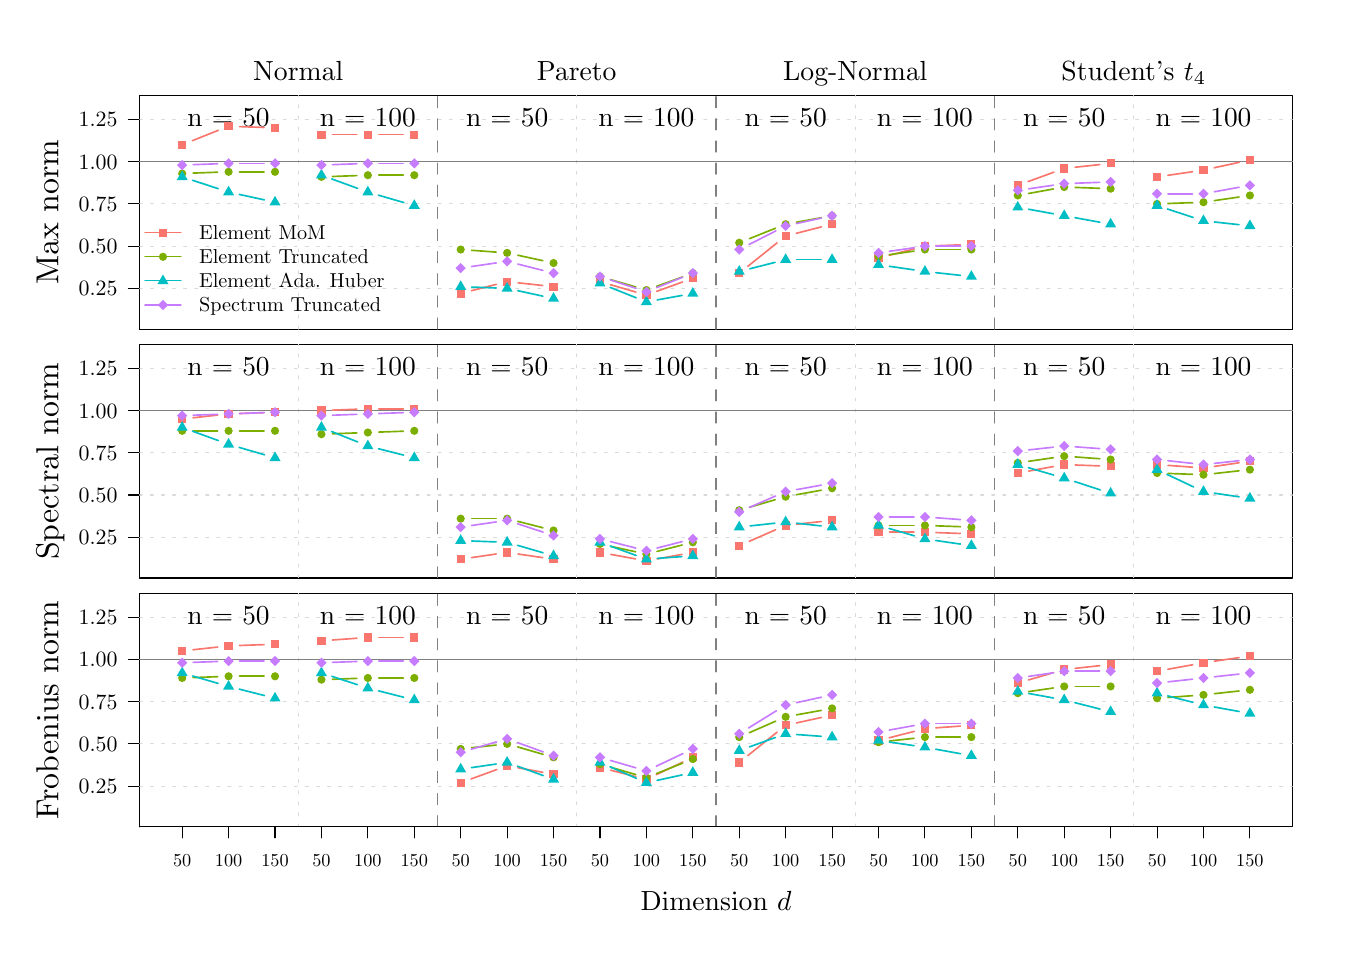
\begin{tikzpicture}[x=1pt,y=1pt]
\definecolor{fillColor}{RGB}{255,255,255}
\path[use as bounding box,fill=fillColor,fill opacity=0.00] (0,0) rectangle (469.76,325.21);
\begin{scope}
\path[clip] (  0.00,  0.00) rectangle (469.76,325.21);
\definecolor{drawColor}{RGB}{0,0,0}

\path[draw=drawColor,line width= 0.4pt,line join=round,line cap=round] ( 40.39,216.28) --
	(457.08,216.28) --
	(457.08,300.66) --
	( 40.39,300.66) --
	( 40.39,216.28);

\path[draw=drawColor,line width= 0.4pt,line join=round,line cap=round] ( 40.39,231.00) -- ( 40.39,292.04);

\path[draw=drawColor,line width= 0.4pt,line join=round,line cap=round] ( 40.39,231.00) -- ( 36.43,231.00);

\path[draw=drawColor,line width= 0.4pt,line join=round,line cap=round] ( 40.39,246.26) -- ( 36.43,246.26);

\path[draw=drawColor,line width= 0.4pt,line join=round,line cap=round] ( 40.39,261.52) -- ( 36.43,261.52);

\path[draw=drawColor,line width= 0.4pt,line join=round,line cap=round] ( 40.39,276.78) -- ( 36.43,276.78);

\path[draw=drawColor,line width= 0.4pt,line join=round,line cap=round] ( 40.39,292.04) -- ( 36.43,292.04);

\node[text=drawColor,anchor=base east,inner sep=0pt, outer sep=0pt, scale=  0.79] at ( 32.47,228.28) {0.25};

\node[text=drawColor,anchor=base east,inner sep=0pt, outer sep=0pt, scale=  0.79] at ( 32.47,243.54) {0.50};

\node[text=drawColor,anchor=base east,inner sep=0pt, outer sep=0pt, scale=  0.79] at ( 32.47,258.80) {0.75};

\node[text=drawColor,anchor=base east,inner sep=0pt, outer sep=0pt, scale=  0.79] at ( 32.47,274.06) {1.00};

\node[text=drawColor,anchor=base east,inner sep=0pt, outer sep=0pt, scale=  0.79] at ( 32.47,289.32) {1.25};
\end{scope}
\begin{scope}
\path[clip] ( 40.39,216.28) rectangle (457.08,300.66);
\definecolor{drawColor}{gray}{0.85}

\path[draw=drawColor,line width= 0.4pt,dash pattern=on 1pt off 3pt ,line join=round,line cap=round] ( 40.39,231.00) -- (457.08,231.00);

\path[draw=drawColor,line width= 0.4pt,dash pattern=on 1pt off 3pt ,line join=round,line cap=round] ( 40.39,246.26) -- (457.08,246.26);

\path[draw=drawColor,line width= 0.4pt,dash pattern=on 1pt off 3pt ,line join=round,line cap=round] ( 40.39,261.52) -- (457.08,261.52);

\path[draw=drawColor,line width= 0.4pt,dash pattern=on 1pt off 3pt ,line join=round,line cap=round] ( 40.39,276.78) -- (457.08,276.78);

\path[draw=drawColor,line width= 0.4pt,dash pattern=on 1pt off 3pt ,line join=round,line cap=round] ( 40.39,292.04) -- (457.08,292.04);

\path[draw=drawColor,line width= 0.4pt,dash pattern=on 1pt off 3pt ,line join=round,line cap=round] ( 97.76,216.28) -- ( 97.76,300.66);

\path[draw=drawColor,line width= 0.4pt,dash pattern=on 1pt off 3pt ,line join=round,line cap=round] (198.41,216.28) -- (198.41,300.66);

\path[draw=drawColor,line width= 0.4pt,dash pattern=on 1pt off 3pt ,line join=round,line cap=round] (299.06,216.28) -- (299.06,300.66);

\path[draw=drawColor,line width= 0.4pt,dash pattern=on 1pt off 3pt ,line join=round,line cap=round] (399.71,216.28) -- (399.71,300.66);
\definecolor{drawColor}{gray}{0.50}

\path[draw=drawColor,line width= 0.4pt,dash pattern=on 4pt off 4pt ,line join=round,line cap=round] (148.09,216.28) -- (148.09,300.66);

\path[draw=drawColor,line width= 0.4pt,dash pattern=on 4pt off 4pt ,line join=round,line cap=round] (248.74,216.28) -- (248.74,300.66);

\path[draw=drawColor,line width= 0.4pt,dash pattern=on 4pt off 4pt ,line join=round,line cap=round] (349.39,216.28) -- (349.39,300.66);
\end{scope}
\begin{scope}
\path[clip] (  0.00,  0.00) rectangle (469.76,325.21);
\definecolor{drawColor}{RGB}{0,0,0}

\node[text=drawColor,rotate= 90.00,anchor=base,inner sep=0pt, outer sep=0pt, scale=  1.15] at ( 11.09,258.47) {Max norm};
\end{scope}
\begin{scope}
\path[clip] ( 40.39,216.28) rectangle (457.08,300.66);
\definecolor{drawColor}{gray}{0.50}

\path[draw=drawColor,line width= 0.4pt,line join=round,line cap=round] ( 40.39,276.78) -- (457.08,276.78);
\end{scope}
\begin{scope}
\path[clip] (  0.00,  0.00) rectangle (469.76,325.21);
\definecolor{drawColor}{RGB}{0,0,0}

\node[text=drawColor,anchor=base,inner sep=0pt, outer sep=0pt, scale=  1.00] at ( 97.76,306.21) {Normal};

\node[text=drawColor,anchor=base,inner sep=0pt, outer sep=0pt, scale=  1.00] at (198.41,306.21) {Pareto};

\node[text=drawColor,anchor=base,inner sep=0pt, outer sep=0pt, scale=  1.00] at (299.06,306.21) {Log-Normal};

\node[text=drawColor,anchor=base,inner sep=0pt, outer sep=0pt, scale=  1.00] at (399.71,306.21) {Student's $t_4$};
\end{scope}
\begin{scope}
\path[clip] ( 40.39,216.28) rectangle (457.08,300.66);
\definecolor{drawColor}{RGB}{0,0,0}

\node[text=drawColor,anchor=base,inner sep=0pt, outer sep=0pt, scale=  0.99] at ( 72.60,289.35) {n = 50};

\node[text=drawColor,anchor=base,inner sep=0pt, outer sep=0pt, scale=  0.99] at (122.92,289.35) {n = 100};

\node[text=drawColor,anchor=base,inner sep=0pt, outer sep=0pt, scale=  0.99] at (173.25,289.35) {n = 50};

\node[text=drawColor,anchor=base,inner sep=0pt, outer sep=0pt, scale=  0.99] at (223.57,289.35) {n = 100};

\node[text=drawColor,anchor=base,inner sep=0pt, outer sep=0pt, scale=  0.99] at (273.90,289.35) {n = 50};

\node[text=drawColor,anchor=base,inner sep=0pt, outer sep=0pt, scale=  0.99] at (324.22,289.35) {n = 100};

\node[text=drawColor,anchor=base,inner sep=0pt, outer sep=0pt, scale=  0.99] at (374.55,289.35) {n = 50};

\node[text=drawColor,anchor=base,inner sep=0pt, outer sep=0pt, scale=  0.99] at (424.87,289.35) {n = 100};
\definecolor{drawColor}{RGB}{248,118,109}

\path[draw=drawColor,line width= 0.4pt,line join=round,line cap=round] ( 42.35,251.13) -- ( 55.42,251.13);
\definecolor{drawColor}{RGB}{124,174,0}

\path[draw=drawColor,line width= 0.4pt,line join=round,line cap=round] ( 42.35,242.42) -- ( 55.42,242.42);
\definecolor{drawColor}{RGB}{0,191,196}

\path[draw=drawColor,line width= 0.4pt,line join=round,line cap=round] ( 42.35,233.71) -- ( 55.42,233.71);
\definecolor{drawColor}{RGB}{199,124,255}

\path[draw=drawColor,line width= 0.4pt,line join=round,line cap=round] ( 42.35,224.99) -- ( 55.42,224.99);
\definecolor{fillColor}{RGB}{248,118,109}

\path[fill=fillColor] ( 47.40,249.64) --
	( 50.37,249.64) --
	( 50.37,252.61) --
	( 47.40,252.61) --
	cycle;
\definecolor{fillColor}{RGB}{124,174,0}

\path[fill=fillColor] ( 48.89,242.42) circle (  1.48);
\definecolor{fillColor}{RGB}{0,191,196}

\path[fill=fillColor] ( 48.89,236.02) --
	( 50.89,232.55) --
	( 46.89,232.55) --
	cycle;
\definecolor{fillColor}{RGB}{199,124,255}

\path[fill=fillColor] ( 47.03,224.99) --
	( 48.89,226.85) --
	( 50.74,224.99) --
	( 48.89,223.14) --
	cycle;
\definecolor{drawColor}{RGB}{0,0,0}

\node[text=drawColor,anchor=base west,inner sep=0pt, outer sep=0pt, scale=  0.73] at ( 61.95,248.63) {Element MoM};

\node[text=drawColor,anchor=base west,inner sep=0pt, outer sep=0pt, scale=  0.73] at ( 61.95,239.92) {Element Truncated};

\node[text=drawColor,anchor=base west,inner sep=0pt, outer sep=0pt, scale=  0.73] at ( 61.95,231.21) {Element Ada. Huber};

\node[text=drawColor,anchor=base west,inner sep=0pt, outer sep=0pt, scale=  0.73] at ( 61.95,222.49) {Spectrum Truncated};
\definecolor{drawColor}{RGB}{248,118,109}

\path[draw=drawColor,line width= 0.6pt,line join=round,line cap=round] ( 59.50,284.36) -- ( 68.92,288.13);

\path[draw=drawColor,line width= 0.6pt,line join=round,line cap=round] ( 76.56,289.46) -- ( 85.42,289.14);
\definecolor{fillColor}{RGB}{248,118,109}

\path[fill=fillColor] ( 54.34,281.40) --
	( 57.31,281.40) --
	( 57.31,284.37) --
	( 54.34,284.37) --
	cycle;

\path[fill=fillColor] ( 71.11,288.12) --
	( 74.08,288.12) --
	( 74.08,291.09) --
	( 71.11,291.09) --
	cycle;

\path[fill=fillColor] ( 87.89,287.51) --
	( 90.86,287.51) --
	( 90.86,290.48) --
	( 87.89,290.48) --
	cycle;
\definecolor{drawColor}{RGB}{124,174,0}

\path[draw=drawColor,line width= 0.6pt,line join=round,line cap=round] ( 59.78,272.66) -- ( 68.64,272.98);

\path[draw=drawColor,line width= 0.6pt,line join=round,line cap=round] ( 76.56,273.12) -- ( 85.42,273.12);
\definecolor{fillColor}{RGB}{124,174,0}

\path[fill=fillColor] ( 55.83,272.51) circle (  1.48);

\path[fill=fillColor] ( 72.60,273.12) circle (  1.48);

\path[fill=fillColor] ( 89.38,273.12) circle (  1.48);
\definecolor{drawColor}{RGB}{0,191,196}

\path[draw=drawColor,line width= 0.6pt,line join=round,line cap=round] ( 59.59,270.06) -- ( 68.84,267.03);

\path[draw=drawColor,line width= 0.6pt,line join=round,line cap=round] ( 76.47,264.95) -- ( 85.51,262.98);
\definecolor{fillColor}{RGB}{0,191,196}

\path[fill=fillColor] ( 55.83,273.60) --
	( 57.82,270.14) --
	( 53.83,270.14) --
	cycle;

\path[fill=fillColor] ( 72.60,268.11) --
	( 74.60,264.64) --
	( 70.60,264.64) --
	cycle;

\path[fill=fillColor] ( 89.38,264.44) --
	( 91.37,260.98) --
	( 87.38,260.98) --
	cycle;
\definecolor{drawColor}{RGB}{199,124,255}

\path[draw=drawColor,line width= 0.6pt,line join=round,line cap=round] ( 59.78,275.71) -- ( 68.64,276.03);

\path[draw=drawColor,line width= 0.6pt,line join=round,line cap=round] ( 76.56,276.17) -- ( 85.42,276.17);
\definecolor{fillColor}{RGB}{199,124,255}

\path[fill=fillColor] ( 53.97,275.56) --
	( 55.83,277.42) --
	( 57.68,275.56) --
	( 55.83,273.71) --
	cycle;

\path[fill=fillColor] ( 70.74,276.17) --
	( 72.60,278.03) --
	( 74.46,276.17) --
	( 72.60,274.32) --
	cycle;

\path[fill=fillColor] ( 87.52,276.17) --
	( 89.38,278.03) --
	( 91.23,276.17) --
	( 89.38,274.32) --
	cycle;
\definecolor{drawColor}{RGB}{248,118,109}

\path[draw=drawColor,line width= 0.6pt,line join=round,line cap=round] (110.11,286.55) -- (118.96,286.55);

\path[draw=drawColor,line width= 0.6pt,line join=round,line cap=round] (126.88,286.55) -- (135.74,286.55);
\definecolor{fillColor}{RGB}{248,118,109}

\path[fill=fillColor] (104.66,285.07) --
	(107.63,285.07) --
	(107.63,288.04) --
	(104.66,288.04) --
	cycle;

\path[fill=fillColor] (121.44,285.07) --
	(124.41,285.07) --
	(124.41,288.04) --
	(121.44,288.04) --
	cycle;

\path[fill=fillColor] (138.21,285.07) --
	(141.19,285.07) --
	(141.19,288.04) --
	(138.21,288.04) --
	cycle;
\definecolor{drawColor}{RGB}{124,174,0}

\path[draw=drawColor,line width= 0.6pt,line join=round,line cap=round] (110.11,271.43) -- (118.97,271.76);

\path[draw=drawColor,line width= 0.6pt,line join=round,line cap=round] (126.88,271.90) -- (135.74,271.90);
\definecolor{fillColor}{RGB}{124,174,0}

\path[fill=fillColor] (106.15,271.29) circle (  1.48);

\path[fill=fillColor] (122.92,271.90) circle (  1.48);

\path[fill=fillColor] (139.70,271.90) circle (  1.48);
\definecolor{drawColor}{RGB}{0,191,196}

\path[draw=drawColor,line width= 0.6pt,line join=round,line cap=round] (109.87,270.55) -- (119.20,267.15);

\path[draw=drawColor,line width= 0.6pt,line join=round,line cap=round] (126.73,264.69) -- (135.90,262.02);
\definecolor{fillColor}{RGB}{0,191,196}

\path[fill=fillColor] (106.15,274.21) --
	(108.15,270.75) --
	(104.15,270.75) --
	cycle;

\path[fill=fillColor] (122.92,268.11) --
	(124.92,264.64) --
	(120.93,264.64) --
	cycle;

\path[fill=fillColor] (139.70,263.22) --
	(141.70,259.76) --
	(137.70,259.76) --
	cycle;
\definecolor{drawColor}{RGB}{199,124,255}

\path[draw=drawColor,line width= 0.6pt,line join=round,line cap=round] (110.11,275.71) -- (118.97,276.03);

\path[draw=drawColor,line width= 0.6pt,line join=round,line cap=round] (126.88,276.17) -- (135.74,276.17);
\definecolor{fillColor}{RGB}{199,124,255}

\path[fill=fillColor] (104.29,275.56) --
	(106.15,277.42) --
	(108.01,275.56) --
	(106.15,273.71) --
	cycle;

\path[fill=fillColor] (121.07,276.17) --
	(122.92,278.03) --
	(124.78,276.17) --
	(122.92,274.32) --
	cycle;

\path[fill=fillColor] (137.84,276.17) --
	(139.70,278.03) --
	(141.56,276.17) --
	(139.70,274.32) --
	cycle;
\definecolor{drawColor}{RGB}{248,118,109}

\path[draw=drawColor,line width= 0.6pt,line join=round,line cap=round] (160.31,230.15) -- (169.41,232.47);

\path[draw=drawColor,line width= 0.6pt,line join=round,line cap=round] (177.19,233.02) -- (186.09,232.04);
\definecolor{fillColor}{RGB}{248,118,109}

\path[fill=fillColor] (154.99,227.69) --
	(157.96,227.69) --
	(157.96,230.66) --
	(154.99,230.66) --
	cycle;

\path[fill=fillColor] (171.76,231.96) --
	(174.73,231.96) --
	(174.73,234.93) --
	(171.76,234.93) --
	cycle;

\path[fill=fillColor] (188.54,230.13) --
	(191.51,230.13) --
	(191.51,233.10) --
	(188.54,233.10) --
	cycle;
\definecolor{drawColor}{RGB}{124,174,0}

\path[draw=drawColor,line width= 0.6pt,line join=round,line cap=round] (160.42,244.76) -- (169.30,244.11);

\path[draw=drawColor,line width= 0.6pt,line join=round,line cap=round] (177.12,242.98) -- (186.16,241.01);
\definecolor{fillColor}{RGB}{124,174,0}

\path[fill=fillColor] (156.47,245.04) circle (  1.48);

\path[fill=fillColor] (173.25,243.82) circle (  1.48);

\path[fill=fillColor] (190.02,240.16) circle (  1.48);
\definecolor{drawColor}{RGB}{0,191,196}

\path[draw=drawColor,line width= 0.6pt,line join=round,line cap=round] (160.43,231.47) -- (169.29,231.15);

\path[draw=drawColor,line width= 0.6pt,line join=round,line cap=round] (177.12,230.16) -- (186.16,228.19);
\definecolor{fillColor}{RGB}{0,191,196}

\path[fill=fillColor] (156.47,233.92) --
	(158.47,230.46) --
	(154.48,230.46) --
	cycle;

\path[fill=fillColor] (173.25,233.31) --
	(175.25,229.85) --
	(171.25,229.85) --
	cycle;

\path[fill=fillColor] (190.02,229.65) --
	(192.02,226.19) --
	(188.03,226.19) --
	cycle;
\definecolor{drawColor}{RGB}{199,124,255}

\path[draw=drawColor,line width= 0.6pt,line join=round,line cap=round] (160.39,238.90) -- (169.33,240.20);

\path[draw=drawColor,line width= 0.6pt,line join=round,line cap=round] (177.09,239.79) -- (186.19,237.48);
\definecolor{fillColor}{RGB}{199,124,255}

\path[fill=fillColor] (154.62,238.33) --
	(156.47,240.19) --
	(158.33,238.33) --
	(156.47,236.47) --
	cycle;

\path[fill=fillColor] (171.39,240.77) --
	(173.25,242.63) --
	(175.11,240.77) --
	(173.25,238.91) --
	cycle;

\path[fill=fillColor] (188.17,236.50) --
	(190.02,238.35) --
	(191.88,236.50) --
	(190.02,234.64) --
	cycle;
\definecolor{drawColor}{RGB}{248,118,109}

\path[draw=drawColor,line width= 0.6pt,line join=round,line cap=round] (210.60,232.34) -- (219.77,229.67);

\path[draw=drawColor,line width= 0.6pt,line join=round,line cap=round] (227.30,229.92) -- (236.63,233.31);
\definecolor{fillColor}{RGB}{248,118,109}

\path[fill=fillColor] (205.31,231.96) --
	(208.28,231.96) --
	(208.28,234.93) --
	(205.31,234.93) --
	cycle;

\path[fill=fillColor] (222.09,227.08) --
	(225.06,227.08) --
	(225.06,230.05) --
	(222.09,230.05) --
	cycle;

\path[fill=fillColor] (238.86,233.18) --
	(241.83,233.18) --
	(241.83,236.15) --
	(238.86,236.15) --
	cycle;
\definecolor{drawColor}{RGB}{124,174,0}

\path[draw=drawColor,line width= 0.6pt,line join=round,line cap=round] (210.60,234.17) -- (219.77,231.50);

\path[draw=drawColor,line width= 0.6pt,line join=round,line cap=round] (227.30,231.75) -- (236.63,235.14);
\definecolor{fillColor}{RGB}{124,174,0}

\path[fill=fillColor] (206.80,235.28) circle (  1.48);

\path[fill=fillColor] (223.57,230.39) circle (  1.48);

\path[fill=fillColor] (240.35,236.50) circle (  1.48);
\definecolor{drawColor}{RGB}{0,191,196}

\path[draw=drawColor,line width= 0.6pt,line join=round,line cap=round] (210.48,231.36) -- (219.90,227.59);

\path[draw=drawColor,line width= 0.6pt,line join=round,line cap=round] (227.47,226.83) -- (236.45,228.46);
\definecolor{fillColor}{RGB}{0,191,196}

\path[fill=fillColor] (206.80,235.15) --
	(208.80,231.68) --
	(204.80,231.68) --
	cycle;

\path[fill=fillColor] (223.57,228.43) --
	(225.57,224.97) --
	(221.58,224.97) --
	cycle;

\path[fill=fillColor] (240.35,231.48) --
	(242.35,228.02) --
	(238.35,228.02) --
	cycle;
\definecolor{drawColor}{RGB}{199,124,255}

\path[draw=drawColor,line width= 0.6pt,line join=round,line cap=round] (210.56,234.05) -- (219.81,231.02);

\path[draw=drawColor,line width= 0.6pt,line join=round,line cap=round] (227.25,231.26) -- (236.67,235.03);
\definecolor{fillColor}{RGB}{199,124,255}

\path[fill=fillColor] (204.94,235.28) --
	(206.80,237.13) --
	(208.66,235.28) --
	(206.80,233.42) --
	cycle;

\path[fill=fillColor] (221.72,229.78) --
	(223.57,231.64) --
	(225.43,229.78) --
	(223.57,227.93) --
	cycle;

\path[fill=fillColor] (238.49,236.50) --
	(240.35,238.35) --
	(242.21,236.50) --
	(240.35,234.64) --
	cycle;
\definecolor{drawColor}{RGB}{248,118,109}

\path[draw=drawColor,line width= 0.6pt,line join=round,line cap=round] (260.22,238.97) -- (270.81,247.45);

\path[draw=drawColor,line width= 0.6pt,line join=round,line cap=round] (277.74,250.90) -- (286.84,253.22);
\definecolor{fillColor}{RGB}{248,118,109}

\path[fill=fillColor] (255.64,235.01) --
	(258.61,235.01) --
	(258.61,237.98) --
	(255.64,237.98) --
	cycle;

\path[fill=fillColor] (272.41,248.44) --
	(275.38,248.44) --
	(275.38,251.41) --
	(272.41,251.41) --
	cycle;

\path[fill=fillColor] (289.19,252.71) --
	(292.16,252.71) --
	(292.16,255.68) --
	(289.19,255.68) --
	cycle;
\definecolor{drawColor}{RGB}{124,174,0}

\path[draw=drawColor,line width= 0.6pt,line join=round,line cap=round] (260.80,248.96) -- (270.22,252.73);

\path[draw=drawColor,line width= 0.6pt,line join=round,line cap=round] (277.80,254.91) -- (286.78,256.54);
\definecolor{fillColor}{RGB}{124,174,0}

\path[fill=fillColor] (257.12,247.49) circle (  1.48);

\path[fill=fillColor] (273.90,254.20) circle (  1.48);

\path[fill=fillColor] (290.67,257.25) circle (  1.48);
\definecolor{drawColor}{RGB}{0,191,196}

\path[draw=drawColor,line width= 0.6pt,line join=round,line cap=round] (260.96,238.09) -- (270.06,240.40);

\path[draw=drawColor,line width= 0.6pt,line join=round,line cap=round] (277.86,241.38) -- (286.71,241.38);
\definecolor{fillColor}{RGB}{0,191,196}

\path[fill=fillColor] (257.12,239.42) --
	(259.12,235.95) --
	(255.13,235.95) --
	cycle;

\path[fill=fillColor] (273.90,243.69) --
	(275.90,240.23) --
	(271.90,240.23) --
	cycle;

\path[fill=fillColor] (290.67,243.69) --
	(292.67,240.23) --
	(288.68,240.23) --
	cycle;
\definecolor{drawColor}{RGB}{199,124,255}

\path[draw=drawColor,line width= 0.6pt,line join=round,line cap=round] (260.65,246.84) -- (270.37,251.79);

\path[draw=drawColor,line width= 0.6pt,line join=round,line cap=round] (277.77,254.43) -- (286.81,256.41);
\definecolor{fillColor}{RGB}{199,124,255}

\path[fill=fillColor] (255.27,245.04) --
	(257.12,246.90) --
	(258.98,245.04) --
	(257.12,243.19) --
	cycle;

\path[fill=fillColor] (272.04,253.59) --
	(273.90,255.45) --
	(275.76,253.59) --
	(273.90,251.73) --
	cycle;

\path[fill=fillColor] (288.82,257.25) --
	(290.67,259.11) --
	(292.53,257.25) --
	(290.67,255.40) --
	cycle;
\definecolor{drawColor}{RGB}{248,118,109}

\path[draw=drawColor,line width= 0.6pt,line join=round,line cap=round] (311.29,242.97) -- (320.39,245.29);

\path[draw=drawColor,line width= 0.6pt,line join=round,line cap=round] (328.18,246.41) -- (337.04,246.73);
\definecolor{fillColor}{RGB}{248,118,109}

\path[fill=fillColor] (305.96,240.51) --
	(308.93,240.51) --
	(308.93,243.48) --
	(305.96,243.48) --
	cycle;

\path[fill=fillColor] (322.74,244.78) --
	(325.71,244.78) --
	(325.71,247.75) --
	(322.74,247.75) --
	cycle;

\path[fill=fillColor] (339.51,245.39) --
	(342.48,245.39) --
	(342.48,248.36) --
	(339.51,248.36) --
	cycle;
\definecolor{drawColor}{RGB}{124,174,0}

\path[draw=drawColor,line width= 0.6pt,line join=round,line cap=round] (311.37,243.17) -- (320.31,244.47);

\path[draw=drawColor,line width= 0.6pt,line join=round,line cap=round] (328.18,245.04) -- (337.04,245.04);
\definecolor{fillColor}{RGB}{124,174,0}

\path[fill=fillColor] (307.45,242.60) circle (  1.48);

\path[fill=fillColor] (324.22,245.04) circle (  1.48);

\path[fill=fillColor] (341.00,245.04) circle (  1.48);
\definecolor{drawColor}{RGB}{0,191,196}

\path[draw=drawColor,line width= 0.6pt,line join=round,line cap=round] (311.37,238.98) -- (320.31,237.68);

\path[draw=drawColor,line width= 0.6pt,line join=round,line cap=round] (328.16,236.68) -- (337.06,235.71);
\definecolor{fillColor}{RGB}{0,191,196}

\path[fill=fillColor] (307.45,241.86) --
	(309.45,238.40) --
	(305.45,238.40) --
	cycle;

\path[fill=fillColor] (324.22,239.42) --
	(326.22,235.95) --
	(322.23,235.95) --
	cycle;

\path[fill=fillColor] (341.00,237.59) --
	(343.00,234.12) --
	(339.00,234.12) --
	cycle;
\definecolor{drawColor}{RGB}{199,124,255}

\path[draw=drawColor,line width= 0.6pt,line join=round,line cap=round] (311.37,244.39) -- (320.31,245.69);

\path[draw=drawColor,line width= 0.6pt,line join=round,line cap=round] (328.18,246.26) -- (337.04,246.26);
\definecolor{fillColor}{RGB}{199,124,255}

\path[fill=fillColor] (305.59,243.82) --
	(307.45,245.68) --
	(309.31,243.82) --
	(307.45,241.97) --
	cycle;

\path[fill=fillColor] (322.37,246.26) --
	(324.22,248.12) --
	(326.08,246.26) --
	(324.22,244.41) --
	cycle;

\path[fill=fillColor] (339.14,246.26) --
	(341.00,248.12) --
	(342.86,246.26) --
	(341.00,244.41) --
	cycle;
\definecolor{drawColor}{RGB}{248,118,109}

\path[draw=drawColor,line width= 0.6pt,line join=round,line cap=round] (361.50,269.59) -- (370.83,272.99);

\path[draw=drawColor,line width= 0.6pt,line join=round,line cap=round] (378.49,274.77) -- (387.39,275.74);
\definecolor{fillColor}{RGB}{248,118,109}

\path[fill=fillColor] (356.29,266.75) --
	(359.26,266.75) --
	(359.26,269.72) --
	(356.29,269.72) --
	cycle;

\path[fill=fillColor] (373.06,272.86) --
	(376.03,272.86) --
	(376.03,275.83) --
	(373.06,275.83) --
	cycle;

\path[fill=fillColor] (389.84,274.69) --
	(392.81,274.69) --
	(392.81,277.66) --
	(389.84,277.66) --
	cycle;
\definecolor{drawColor}{RGB}{124,174,0}

\path[draw=drawColor,line width= 0.6pt,line join=round,line cap=round] (361.67,265.29) -- (370.65,266.92);

\path[draw=drawColor,line width= 0.6pt,line join=round,line cap=round] (378.51,267.48) -- (387.37,267.16);
\definecolor{fillColor}{RGB}{124,174,0}

\path[fill=fillColor] (357.77,264.58) circle (  1.48);

\path[fill=fillColor] (374.55,267.63) circle (  1.48);

\path[fill=fillColor] (391.32,267.02) circle (  1.48);
\definecolor{drawColor}{RGB}{0,191,196}

\path[draw=drawColor,line width= 0.6pt,line join=round,line cap=round] (361.67,259.59) -- (370.65,257.96);

\path[draw=drawColor,line width= 0.6pt,line join=round,line cap=round] (378.45,256.54) -- (387.43,254.91);
\definecolor{fillColor}{RGB}{0,191,196}

\path[fill=fillColor] (357.77,262.61) --
	(359.77,259.15) --
	(355.78,259.15) --
	cycle;

\path[fill=fillColor] (374.55,259.56) --
	(376.55,256.10) --
	(372.55,256.10) --
	cycle;

\path[fill=fillColor] (391.32,256.51) --
	(393.32,253.05) --
	(389.33,253.05) --
	cycle;
\definecolor{drawColor}{RGB}{199,124,255}

\path[draw=drawColor,line width= 0.6pt,line join=round,line cap=round] (361.69,266.98) -- (370.63,268.28);

\path[draw=drawColor,line width= 0.6pt,line join=round,line cap=round] (378.51,268.99) -- (387.37,269.32);
\definecolor{fillColor}{RGB}{199,124,255}

\path[fill=fillColor] (355.92,266.41) --
	(357.77,268.26) --
	(359.63,266.41) --
	(357.77,264.55) --
	cycle;

\path[fill=fillColor] (372.69,268.85) --
	(374.55,270.71) --
	(376.41,268.85) --
	(374.55,266.99) --
	cycle;

\path[fill=fillColor] (389.47,269.46) --
	(391.32,271.32) --
	(393.18,269.46) --
	(391.32,267.60) --
	cycle;
\definecolor{drawColor}{RGB}{248,118,109}

\path[draw=drawColor,line width= 0.6pt,line join=round,line cap=round] (412.02,271.86) -- (420.96,273.16);

\path[draw=drawColor,line width= 0.6pt,line join=round,line cap=round] (428.74,274.58) -- (437.78,276.55);
\definecolor{fillColor}{RGB}{248,118,109}

\path[fill=fillColor] (406.61,269.81) --
	(409.58,269.81) --
	(409.58,272.78) --
	(406.61,272.78) --
	cycle;

\path[fill=fillColor] (423.39,272.25) --
	(426.36,272.25) --
	(426.36,275.22) --
	(423.39,275.22) --
	cycle;

\path[fill=fillColor] (440.16,275.91) --
	(443.13,275.91) --
	(443.13,278.88) --
	(440.16,278.88) --
	cycle;
\definecolor{drawColor}{RGB}{124,174,0}

\path[draw=drawColor,line width= 0.6pt,line join=round,line cap=round] (412.06,261.67) -- (420.92,261.99);

\path[draw=drawColor,line width= 0.6pt,line join=round,line cap=round] (428.79,262.71) -- (437.73,264.01);
\definecolor{fillColor}{RGB}{124,174,0}

\path[fill=fillColor] (408.10,261.52) circle (  1.48);

\path[fill=fillColor] (424.87,262.13) circle (  1.48);

\path[fill=fillColor] (441.65,264.58) circle (  1.48);
\definecolor{drawColor}{RGB}{0,191,196}

\path[draw=drawColor,line width= 0.6pt,line join=round,line cap=round] (411.86,259.68) -- (421.11,256.65);

\path[draw=drawColor,line width= 0.6pt,line join=round,line cap=round] (428.81,254.99) -- (437.71,254.02);
\definecolor{fillColor}{RGB}{0,191,196}

\path[fill=fillColor] (408.10,263.22) --
	(410.10,259.76) --
	(406.10,259.76) --
	cycle;

\path[fill=fillColor] (424.87,257.73) --
	(426.87,254.27) --
	(422.88,254.27) --
	cycle;

\path[fill=fillColor] (441.65,255.90) --
	(443.65,252.43) --
	(439.65,252.43) --
	cycle;
\definecolor{drawColor}{RGB}{199,124,255}

\path[draw=drawColor,line width= 0.6pt,line join=round,line cap=round] (412.06,265.19) -- (420.91,265.19);

\path[draw=drawColor,line width= 0.6pt,line join=round,line cap=round] (428.77,265.90) -- (437.75,267.53);
\definecolor{fillColor}{RGB}{199,124,255}

\path[fill=fillColor] (406.24,265.19) --
	(408.10,267.04) --
	(409.96,265.19) --
	(408.10,263.33) --
	cycle;

\path[fill=fillColor] (423.02,265.19) --
	(424.87,267.04) --
	(426.73,265.19) --
	(424.87,263.33) --
	cycle;

\path[fill=fillColor] (439.79,268.24) --
	(441.65,270.10) --
	(443.51,268.24) --
	(441.65,266.38) --
	cycle;
\end{scope}
\begin{scope}
\path[clip] (  0.00,  0.00) rectangle (469.76,325.21);
\definecolor{drawColor}{RGB}{0,0,0}

\path[draw=drawColor,line width= 0.4pt,line join=round,line cap=round] ( 40.39,126.36) --
	(457.08,126.36) --
	(457.08,210.74) --
	( 40.39,210.74) --
	( 40.39,126.36);

\path[draw=drawColor,line width= 0.4pt,line join=round,line cap=round] ( 40.39,141.08) -- ( 40.39,202.12);

\path[draw=drawColor,line width= 0.4pt,line join=round,line cap=round] ( 40.39,141.08) -- ( 36.43,141.08);

\path[draw=drawColor,line width= 0.4pt,line join=round,line cap=round] ( 40.39,156.34) -- ( 36.43,156.34);

\path[draw=drawColor,line width= 0.4pt,line join=round,line cap=round] ( 40.39,171.60) -- ( 36.43,171.60);

\path[draw=drawColor,line width= 0.4pt,line join=round,line cap=round] ( 40.39,186.86) -- ( 36.43,186.86);

\path[draw=drawColor,line width= 0.4pt,line join=round,line cap=round] ( 40.39,202.12) -- ( 36.43,202.12);

\node[text=drawColor,anchor=base east,inner sep=0pt, outer sep=0pt, scale=  0.79] at ( 32.47,138.35) {0.25};

\node[text=drawColor,anchor=base east,inner sep=0pt, outer sep=0pt, scale=  0.79] at ( 32.47,153.61) {0.50};

\node[text=drawColor,anchor=base east,inner sep=0pt, outer sep=0pt, scale=  0.79] at ( 32.47,168.87) {0.75};

\node[text=drawColor,anchor=base east,inner sep=0pt, outer sep=0pt, scale=  0.79] at ( 32.47,184.13) {1.00};

\node[text=drawColor,anchor=base east,inner sep=0pt, outer sep=0pt, scale=  0.79] at ( 32.47,199.39) {1.25};
\end{scope}
\begin{scope}
\path[clip] ( 40.39,126.36) rectangle (457.08,210.74);
\definecolor{drawColor}{gray}{0.85}

\path[draw=drawColor,line width= 0.4pt,dash pattern=on 1pt off 3pt ,line join=round,line cap=round] ( 40.39,141.08) -- (457.08,141.08);

\path[draw=drawColor,line width= 0.4pt,dash pattern=on 1pt off 3pt ,line join=round,line cap=round] ( 40.39,156.34) -- (457.08,156.34);

\path[draw=drawColor,line width= 0.4pt,dash pattern=on 1pt off 3pt ,line join=round,line cap=round] ( 40.39,171.60) -- (457.08,171.60);

\path[draw=drawColor,line width= 0.4pt,dash pattern=on 1pt off 3pt ,line join=round,line cap=round] ( 40.39,186.86) -- (457.08,186.86);

\path[draw=drawColor,line width= 0.4pt,dash pattern=on 1pt off 3pt ,line join=round,line cap=round] ( 40.39,202.12) -- (457.08,202.12);

\path[draw=drawColor,line width= 0.4pt,dash pattern=on 1pt off 3pt ,line join=round,line cap=round] ( 97.76,126.36) -- ( 97.76,210.74);

\path[draw=drawColor,line width= 0.4pt,dash pattern=on 1pt off 3pt ,line join=round,line cap=round] (198.41,126.36) -- (198.41,210.74);

\path[draw=drawColor,line width= 0.4pt,dash pattern=on 1pt off 3pt ,line join=round,line cap=round] (299.06,126.36) -- (299.06,210.74);

\path[draw=drawColor,line width= 0.4pt,dash pattern=on 1pt off 3pt ,line join=round,line cap=round] (399.71,126.36) -- (399.71,210.74);
\definecolor{drawColor}{gray}{0.50}

\path[draw=drawColor,line width= 0.4pt,dash pattern=on 4pt off 4pt ,line join=round,line cap=round] (148.09,126.36) -- (148.09,210.74);

\path[draw=drawColor,line width= 0.4pt,dash pattern=on 4pt off 4pt ,line join=round,line cap=round] (248.74,126.36) -- (248.74,210.74);

\path[draw=drawColor,line width= 0.4pt,dash pattern=on 4pt off 4pt ,line join=round,line cap=round] (349.39,126.36) -- (349.39,210.74);
\end{scope}
\begin{scope}
\path[clip] (  0.00,  0.00) rectangle (469.76,325.21);
\definecolor{drawColor}{RGB}{0,0,0}

\node[text=drawColor,rotate= 90.00,anchor=base,inner sep=0pt, outer sep=0pt, scale=  1.15] at ( 11.09,168.55) {Spectral norm};
\end{scope}
\begin{scope}
\path[clip] ( 40.39,126.36) rectangle (457.08,210.74);
\definecolor{drawColor}{gray}{0.50}

\path[draw=drawColor,line width= 0.4pt,line join=round,line cap=round] ( 40.39,186.86) -- (457.08,186.86);
\definecolor{drawColor}{RGB}{0,0,0}

\node[text=drawColor,anchor=base,inner sep=0pt, outer sep=0pt, scale=  0.99] at ( 72.60,199.42) {n = 50};

\node[text=drawColor,anchor=base,inner sep=0pt, outer sep=0pt, scale=  0.99] at (122.92,199.42) {n = 100};

\node[text=drawColor,anchor=base,inner sep=0pt, outer sep=0pt, scale=  0.99] at (173.25,199.42) {n = 50};

\node[text=drawColor,anchor=base,inner sep=0pt, outer sep=0pt, scale=  0.99] at (223.57,199.42) {n = 100};

\node[text=drawColor,anchor=base,inner sep=0pt, outer sep=0pt, scale=  0.99] at (273.90,199.42) {n = 50};

\node[text=drawColor,anchor=base,inner sep=0pt, outer sep=0pt, scale=  0.99] at (324.22,199.42) {n = 100};

\node[text=drawColor,anchor=base,inner sep=0pt, outer sep=0pt, scale=  0.99] at (374.55,199.42) {n = 50};

\node[text=drawColor,anchor=base,inner sep=0pt, outer sep=0pt, scale=  0.99] at (424.87,199.42) {n = 100};
\definecolor{drawColor}{RGB}{248,118,109}

\path[draw=drawColor,line width= 0.6pt,line join=round,line cap=round] ( 59.76,184.24) -- ( 68.66,185.21);

\path[draw=drawColor,line width= 0.6pt,line join=round,line cap=round] ( 76.56,185.78) -- ( 85.42,186.10);
\definecolor{fillColor}{RGB}{248,118,109}

\path[fill=fillColor] ( 54.34,182.32) --
	( 57.31,182.32) --
	( 57.31,185.29) --
	( 54.34,185.29) --
	cycle;

\path[fill=fillColor] ( 71.11,184.15) --
	( 74.08,184.15) --
	( 74.08,187.12) --
	( 71.11,187.12) --
	cycle;

\path[fill=fillColor] ( 87.89,184.76) --
	( 90.86,184.76) --
	( 90.86,187.73) --
	( 87.89,187.73) --
	cycle;
\definecolor{drawColor}{RGB}{124,174,0}

\path[draw=drawColor,line width= 0.6pt,line join=round,line cap=round] ( 59.79,179.53) -- ( 68.64,179.53);

\path[draw=drawColor,line width= 0.6pt,line join=round,line cap=round] ( 76.56,179.53) -- ( 85.42,179.53);
\definecolor{fillColor}{RGB}{124,174,0}

\path[fill=fillColor] ( 55.83,179.53) circle (  1.48);

\path[fill=fillColor] ( 72.60,179.53) circle (  1.48);

\path[fill=fillColor] ( 89.38,179.53) circle (  1.48);
\definecolor{drawColor}{RGB}{0,191,196}

\path[draw=drawColor,line width= 0.6pt,line join=round,line cap=round] ( 59.55,179.40) -- ( 68.88,176.01);

\path[draw=drawColor,line width= 0.6pt,line join=round,line cap=round] ( 76.40,173.54) -- ( 85.57,170.88);
\definecolor{fillColor}{RGB}{0,191,196}

\path[fill=fillColor] ( 55.83,183.06) --
	( 57.82,179.60) --
	( 53.83,179.60) --
	cycle;

\path[fill=fillColor] ( 72.60,176.96) --
	( 74.60,173.50) --
	( 70.60,173.50) --
	cycle;

\path[fill=fillColor] ( 89.38,172.08) --
	( 91.37,168.61) --
	( 87.38,168.61) --
	cycle;
\definecolor{drawColor}{RGB}{199,124,255}

\path[draw=drawColor,line width= 0.6pt,line join=round,line cap=round] ( 59.78,185.17) -- ( 68.64,185.49);

\path[draw=drawColor,line width= 0.6pt,line join=round,line cap=round] ( 76.56,185.78) -- ( 85.42,186.10);
\definecolor{fillColor}{RGB}{199,124,255}

\path[fill=fillColor] ( 53.97,185.03) --
	( 55.83,186.88) --
	( 57.68,185.03) --
	( 55.83,183.17) --
	cycle;

\path[fill=fillColor] ( 70.74,185.64) --
	( 72.60,187.49) --
	( 74.46,185.64) --
	( 72.60,183.78) --
	cycle;

\path[fill=fillColor] ( 87.52,186.25) --
	( 89.38,188.11) --
	( 91.23,186.25) --
	( 89.38,184.39) --
	cycle;
\definecolor{drawColor}{RGB}{248,118,109}

\path[draw=drawColor,line width= 0.6pt,line join=round,line cap=round] (110.11,187.00) -- (118.97,187.33);

\path[draw=drawColor,line width= 0.6pt,line join=round,line cap=round] (126.88,187.47) -- (135.74,187.47);
\definecolor{fillColor}{RGB}{248,118,109}

\path[fill=fillColor] (104.66,185.37) --
	(107.63,185.37) --
	(107.63,188.34) --
	(104.66,188.34) --
	cycle;

\path[fill=fillColor] (121.44,185.98) --
	(124.41,185.98) --
	(124.41,188.95) --
	(121.44,188.95) --
	cycle;

\path[fill=fillColor] (138.21,185.98) --
	(141.19,185.98) --
	(141.19,188.95) --
	(138.21,188.95) --
	cycle;
\definecolor{drawColor}{RGB}{124,174,0}

\path[draw=drawColor,line width= 0.6pt,line join=round,line cap=round] (110.11,178.46) -- (118.97,178.78);

\path[draw=drawColor,line width= 0.6pt,line join=round,line cap=round] (126.88,179.07) -- (135.74,179.39);
\definecolor{fillColor}{RGB}{124,174,0}

\path[fill=fillColor] (106.15,178.31) circle (  1.48);

\path[fill=fillColor] (122.92,178.92) circle (  1.48);

\path[fill=fillColor] (139.70,179.53) circle (  1.48);
\definecolor{drawColor}{RGB}{0,191,196}

\path[draw=drawColor,line width= 0.6pt,line join=round,line cap=round] (109.83,179.28) -- (119.25,175.51);

\path[draw=drawColor,line width= 0.6pt,line join=round,line cap=round] (126.76,173.06) -- (135.86,170.75);
\definecolor{fillColor}{RGB}{0,191,196}

\path[fill=fillColor] (106.15,183.06) --
	(108.15,179.60) --
	(104.15,179.60) --
	cycle;

\path[fill=fillColor] (122.92,176.35) --
	(124.92,172.89) --
	(120.93,172.89) --
	cycle;

\path[fill=fillColor] (139.70,172.08) --
	(141.70,168.61) --
	(137.70,168.61) --
	cycle;
\definecolor{drawColor}{RGB}{199,124,255}

\path[draw=drawColor,line width= 0.6pt,line join=round,line cap=round] (110.11,185.17) -- (118.97,185.49);

\path[draw=drawColor,line width= 0.6pt,line join=round,line cap=round] (126.88,185.78) -- (135.74,186.10);
\definecolor{fillColor}{RGB}{199,124,255}

\path[fill=fillColor] (104.29,185.03) --
	(106.15,186.88) --
	(108.01,185.03) --
	(106.15,183.17) --
	cycle;

\path[fill=fillColor] (121.07,185.64) --
	(122.92,187.49) --
	(124.78,185.64) --
	(122.92,183.78) --
	cycle;

\path[fill=fillColor] (137.84,186.25) --
	(139.70,188.11) --
	(141.56,186.25) --
	(139.70,184.39) --
	cycle;
\definecolor{drawColor}{RGB}{248,118,109}

\path[draw=drawColor,line width= 0.6pt,line join=round,line cap=round] (160.39,133.71) -- (169.33,135.02);

\path[draw=drawColor,line width= 0.6pt,line join=round,line cap=round] (177.17,135.02) -- (186.11,133.71);
\definecolor{fillColor}{RGB}{248,118,109}

\path[fill=fillColor] (154.99,131.66) --
	(157.96,131.66) --
	(157.96,134.63) --
	(154.99,134.63) --
	cycle;

\path[fill=fillColor] (171.76,134.10) --
	(174.73,134.10) --
	(174.73,137.07) --
	(171.76,137.07) --
	cycle;

\path[fill=fillColor] (188.54,131.66) --
	(191.51,131.66) --
	(191.51,134.63) --
	(188.54,134.63) --
	cycle;
\definecolor{drawColor}{RGB}{124,174,0}

\path[draw=drawColor,line width= 0.6pt,line join=round,line cap=round] (160.44,147.79) -- (169.29,147.79);

\path[draw=drawColor,line width= 0.6pt,line join=round,line cap=round] (177.09,146.82) -- (186.19,144.50);
\definecolor{fillColor}{RGB}{124,174,0}

\path[fill=fillColor] (156.47,147.79) circle (  1.48);

\path[fill=fillColor] (173.25,147.79) circle (  1.48);

\path[fill=fillColor] (190.02,143.52) circle (  1.48);
\definecolor{drawColor}{RGB}{0,191,196}

\path[draw=drawColor,line width= 0.6pt,line join=round,line cap=round] (160.43,139.71) -- (169.29,139.39);

\path[draw=drawColor,line width= 0.6pt,line join=round,line cap=round] (177.05,138.14) -- (186.22,135.47);
\definecolor{fillColor}{RGB}{0,191,196}

\path[fill=fillColor] (156.47,142.17) --
	(158.47,138.70) --
	(154.48,138.70) --
	cycle;

\path[fill=fillColor] (173.25,141.56) --
	(175.25,138.09) --
	(171.25,138.09) --
	cycle;

\path[fill=fillColor] (190.02,136.67) --
	(192.02,133.21) --
	(188.03,133.21) --
	cycle;
\definecolor{drawColor}{RGB}{199,124,255}

\path[draw=drawColor,line width= 0.6pt,line join=round,line cap=round] (160.39,145.31) -- (169.33,146.61);

\path[draw=drawColor,line width= 0.6pt,line join=round,line cap=round] (177.01,145.95) -- (186.26,142.92);
\definecolor{fillColor}{RGB}{199,124,255}

\path[fill=fillColor] (154.62,144.74) --
	(156.47,146.60) --
	(158.33,144.74) --
	(156.47,142.89) --
	cycle;

\path[fill=fillColor] (171.39,147.18) --
	(173.25,149.04) --
	(175.11,147.18) --
	(173.25,145.33) --
	cycle;

\path[fill=fillColor] (188.17,141.69) --
	(190.02,143.55) --
	(191.88,141.69) --
	(190.02,139.83) --
	cycle;
\definecolor{drawColor}{RGB}{248,118,109}

\path[draw=drawColor,line width= 0.6pt,line join=round,line cap=round] (210.70,134.88) -- (219.68,133.24);

\path[draw=drawColor,line width= 0.6pt,line join=round,line cap=round] (227.47,133.24) -- (236.45,134.88);
\definecolor{fillColor}{RGB}{248,118,109}

\path[fill=fillColor] (205.31,134.10) --
	(208.28,134.10) --
	(208.28,137.07) --
	(205.31,137.07) --
	cycle;

\path[fill=fillColor] (222.09,131.05) --
	(225.06,131.05) --
	(225.06,134.02) --
	(222.09,134.02) --
	cycle;

\path[fill=fillColor] (238.86,134.10) --
	(241.83,134.10) --
	(241.83,137.07) --
	(238.86,137.07) --
	cycle;
\definecolor{drawColor}{RGB}{124,174,0}

\path[draw=drawColor,line width= 0.6pt,line join=round,line cap=round] (210.67,137.79) -- (219.71,135.82);

\path[draw=drawColor,line width= 0.6pt,line join=round,line cap=round] (227.41,135.95) -- (236.51,138.27);
\definecolor{fillColor}{RGB}{124,174,0}

\path[fill=fillColor] (206.80,138.64) circle (  1.48);

\path[fill=fillColor] (223.57,134.98) circle (  1.48);

\path[fill=fillColor] (240.35,139.25) circle (  1.48);
\definecolor{drawColor}{RGB}{0,191,196}

\path[draw=drawColor,line width= 0.6pt,line join=round,line cap=round] (210.52,137.89) -- (219.85,134.50);

\path[draw=drawColor,line width= 0.6pt,line join=round,line cap=round] (227.52,133.43) -- (236.40,134.08);
\definecolor{fillColor}{RGB}{0,191,196}

\path[fill=fillColor] (206.80,141.56) --
	(208.80,138.09) --
	(204.80,138.09) --
	cycle;

\path[fill=fillColor] (223.57,135.45) --
	(225.57,131.99) --
	(221.58,131.99) --
	cycle;

\path[fill=fillColor] (240.35,136.67) --
	(242.35,133.21) --
	(238.35,133.21) --
	cycle;
\definecolor{drawColor}{RGB}{199,124,255}

\path[draw=drawColor,line width= 0.6pt,line join=round,line cap=round] (210.64,139.49) -- (219.74,137.17);

\path[draw=drawColor,line width= 0.6pt,line join=round,line cap=round] (227.41,137.17) -- (236.51,139.49);
\definecolor{fillColor}{RGB}{199,124,255}

\path[fill=fillColor] (204.94,140.47) --
	(206.80,142.33) --
	(208.66,140.47) --
	(206.80,138.61) --
	cycle;

\path[fill=fillColor] (221.72,136.20) --
	(223.57,138.05) --
	(225.43,136.20) --
	(223.57,134.34) --
	cycle;

\path[fill=fillColor] (238.49,140.47) --
	(240.35,142.33) --
	(242.21,140.47) --
	(240.35,138.61) --
	cycle;
\definecolor{drawColor}{RGB}{248,118,109}

\path[draw=drawColor,line width= 0.6pt,line join=round,line cap=round] (260.75,139.61) -- (270.27,143.77);

\path[draw=drawColor,line width= 0.6pt,line join=round,line cap=round] (277.84,145.78) -- (286.74,146.75);
\definecolor{fillColor}{RGB}{248,118,109}

\path[fill=fillColor] (255.64,136.54) --
	(258.61,136.54) --
	(258.61,139.51) --
	(255.64,139.51) --
	cycle;

\path[fill=fillColor] (272.41,143.87) --
	(275.38,143.87) --
	(275.38,146.84) --
	(272.41,146.84) --
	cycle;

\path[fill=fillColor] (289.19,145.70) --
	(292.16,145.70) --
	(292.16,148.67) --
	(289.19,148.67) --
	cycle;
\definecolor{drawColor}{RGB}{124,174,0}

\path[draw=drawColor,line width= 0.6pt,line join=round,line cap=round] (260.93,151.95) -- (270.10,154.62);

\path[draw=drawColor,line width= 0.6pt,line join=round,line cap=round] (277.80,156.44) -- (286.78,158.07);
\definecolor{fillColor}{RGB}{124,174,0}

\path[fill=fillColor] (257.12,150.85) circle (  1.48);

\path[fill=fillColor] (273.90,155.73) circle (  1.48);

\path[fill=fillColor] (290.67,158.78) circle (  1.48);
\definecolor{drawColor}{RGB}{0,191,196}

\path[draw=drawColor,line width= 0.6pt,line join=round,line cap=round] (261.06,145.17) -- (269.96,146.14);

\path[draw=drawColor,line width= 0.6pt,line join=round,line cap=round] (277.84,146.14) -- (286.74,145.17);
\definecolor{fillColor}{RGB}{0,191,196}

\path[fill=fillColor] (257.12,147.05) --
	(259.12,143.59) --
	(255.13,143.59) --
	cycle;

\path[fill=fillColor] (273.90,148.88) --
	(275.90,145.42) --
	(271.90,145.42) --
	cycle;

\path[fill=fillColor] (290.67,147.05) --
	(292.67,143.59) --
	(288.68,143.59) --
	cycle;
\definecolor{drawColor}{RGB}{199,124,255}

\path[draw=drawColor,line width= 0.6pt,line join=round,line cap=round] (260.75,151.82) -- (270.27,155.98);

\path[draw=drawColor,line width= 0.6pt,line join=round,line cap=round] (277.80,158.27) -- (286.78,159.90);
\definecolor{fillColor}{RGB}{199,124,255}

\path[fill=fillColor] (255.27,150.24) --
	(257.12,152.09) --
	(258.98,150.24) --
	(257.12,148.38) --
	cycle;

\path[fill=fillColor] (272.04,157.56) --
	(273.90,159.42) --
	(275.76,157.56) --
	(273.90,155.70) --
	cycle;

\path[fill=fillColor] (288.82,160.61) --
	(290.67,162.47) --
	(292.53,160.61) --
	(290.67,158.76) --
	cycle;
\definecolor{drawColor}{RGB}{248,118,109}

\path[draw=drawColor,line width= 0.6pt,line join=round,line cap=round] (311.41,142.91) -- (320.26,142.91);

\path[draw=drawColor,line width= 0.6pt,line join=round,line cap=round] (328.18,142.77) -- (337.04,142.44);
\definecolor{fillColor}{RGB}{248,118,109}

\path[fill=fillColor] (305.96,141.43) --
	(308.93,141.43) --
	(308.93,144.40) --
	(305.96,144.40) --
	cycle;

\path[fill=fillColor] (322.74,141.43) --
	(325.71,141.43) --
	(325.71,144.40) --
	(322.74,144.40) --
	cycle;

\path[fill=fillColor] (339.51,140.82) --
	(342.48,140.82) --
	(342.48,143.79) --
	(339.51,143.79) --
	cycle;
\definecolor{drawColor}{RGB}{124,174,0}

\path[draw=drawColor,line width= 0.6pt,line join=round,line cap=round] (311.41,145.35) -- (320.26,145.35);

\path[draw=drawColor,line width= 0.6pt,line join=round,line cap=round] (328.18,145.21) -- (337.04,144.89);
\definecolor{fillColor}{RGB}{124,174,0}

\path[fill=fillColor] (307.45,145.35) circle (  1.48);

\path[fill=fillColor] (324.22,145.35) circle (  1.48);

\path[fill=fillColor] (341.00,144.74) circle (  1.48);
\definecolor{drawColor}{RGB}{0,191,196}

\path[draw=drawColor,line width= 0.6pt,line join=round,line cap=round] (311.25,144.25) -- (320.42,141.58);

\path[draw=drawColor,line width= 0.6pt,line join=round,line cap=round] (328.14,139.90) -- (337.08,138.60);
\definecolor{fillColor}{RGB}{0,191,196}

\path[fill=fillColor] (307.45,147.66) --
	(309.45,144.20) --
	(305.45,144.20) --
	cycle;

\path[fill=fillColor] (324.22,142.78) --
	(326.22,139.31) --
	(322.23,139.31) --
	cycle;

\path[fill=fillColor] (341.00,140.34) --
	(343.00,136.87) --
	(339.00,136.87) --
	cycle;
\definecolor{drawColor}{RGB}{199,124,255}

\path[draw=drawColor,line width= 0.6pt,line join=round,line cap=round] (311.41,148.40) -- (320.26,148.40);

\path[draw=drawColor,line width= 0.6pt,line join=round,line cap=round] (328.17,148.12) -- (337.05,147.47);
\definecolor{fillColor}{RGB}{199,124,255}

\path[fill=fillColor] (305.59,148.40) --
	(307.45,150.26) --
	(309.31,148.40) --
	(307.45,146.55) --
	cycle;

\path[fill=fillColor] (322.37,148.40) --
	(324.22,150.26) --
	(326.08,148.40) --
	(324.22,146.55) --
	cycle;

\path[fill=fillColor] (339.14,147.18) --
	(341.00,149.04) --
	(342.86,147.18) --
	(341.00,145.33) --
	cycle;
\definecolor{drawColor}{RGB}{248,118,109}

\path[draw=drawColor,line width= 0.6pt,line join=round,line cap=round] (361.67,164.98) -- (370.65,166.62);

\path[draw=drawColor,line width= 0.6pt,line join=round,line cap=round] (378.51,167.18) -- (387.37,166.86);
\definecolor{fillColor}{RGB}{248,118,109}

\path[fill=fillColor] (356.29,162.79) --
	(359.26,162.79) --
	(359.26,165.76) --
	(356.29,165.76) --
	cycle;

\path[fill=fillColor] (373.06,165.84) --
	(376.03,165.84) --
	(376.03,168.81) --
	(373.06,168.81) --
	cycle;

\path[fill=fillColor] (389.84,165.23) --
	(392.81,165.23) --
	(392.81,168.20) --
	(389.84,168.20) --
	cycle;
\definecolor{drawColor}{RGB}{124,174,0}

\path[draw=drawColor,line width= 0.6pt,line join=round,line cap=round] (361.69,168.51) -- (370.63,169.81);

\path[draw=drawColor,line width= 0.6pt,line join=round,line cap=round] (378.50,170.09) -- (387.38,169.45);
\definecolor{fillColor}{RGB}{124,174,0}

\path[fill=fillColor] (357.77,167.94) circle (  1.48);

\path[fill=fillColor] (374.55,170.38) circle (  1.48);

\path[fill=fillColor] (391.32,169.16) circle (  1.48);
\definecolor{drawColor}{RGB}{0,191,196}

\path[draw=drawColor,line width= 0.6pt,line join=round,line cap=round] (361.58,166.22) -- (370.75,163.55);

\path[draw=drawColor,line width= 0.6pt,line join=round,line cap=round] (378.31,161.21) -- (387.56,158.18);
\definecolor{fillColor}{RGB}{0,191,196}

\path[fill=fillColor] (357.77,169.64) --
	(359.77,166.17) --
	(355.78,166.17) --
	cycle;

\path[fill=fillColor] (374.55,164.75) --
	(376.55,161.29) --
	(372.55,161.29) --
	cycle;

\path[fill=fillColor] (391.32,159.26) --
	(393.32,155.80) --
	(389.33,155.80) --
	cycle;
\definecolor{drawColor}{RGB}{199,124,255}

\path[draw=drawColor,line width= 0.6pt,line join=round,line cap=round] (361.71,172.64) -- (370.61,173.61);

\path[draw=drawColor,line width= 0.6pt,line join=round,line cap=round] (378.50,173.75) -- (387.38,173.11);
\definecolor{fillColor}{RGB}{199,124,255}

\path[fill=fillColor] (355.92,172.21) --
	(357.77,174.07) --
	(359.63,172.21) --
	(357.77,170.35) --
	cycle;

\path[fill=fillColor] (372.69,174.04) --
	(374.55,175.90) --
	(376.41,174.04) --
	(374.55,172.18) --
	cycle;

\path[fill=fillColor] (389.47,172.82) --
	(391.32,174.68) --
	(393.18,172.82) --
	(391.32,170.96) --
	cycle;
\definecolor{drawColor}{RGB}{248,118,109}

\path[draw=drawColor,line width= 0.6pt,line join=round,line cap=round] (412.05,167.04) -- (420.93,166.39);

\path[draw=drawColor,line width= 0.6pt,line join=round,line cap=round] (428.79,166.68) -- (437.73,167.98);
\definecolor{fillColor}{RGB}{248,118,109}

\path[fill=fillColor] (406.61,165.84) --
	(409.58,165.84) --
	(409.58,168.81) --
	(406.61,168.81) --
	cycle;

\path[fill=fillColor] (423.39,164.62) --
	(426.36,164.62) --
	(426.36,167.59) --
	(423.39,167.59) --
	cycle;

\path[fill=fillColor] (440.16,167.06) --
	(443.13,167.06) --
	(443.13,170.03) --
	(440.16,170.03) --
	cycle;
\definecolor{drawColor}{RGB}{124,174,0}

\path[draw=drawColor,line width= 0.6pt,line join=round,line cap=round] (412.06,164.13) -- (420.92,163.81);

\path[draw=drawColor,line width= 0.6pt,line join=round,line cap=round] (428.81,164.09) -- (437.71,165.07);
\definecolor{fillColor}{RGB}{124,174,0}

\path[fill=fillColor] (408.10,164.27) circle (  1.48);

\path[fill=fillColor] (424.87,163.66) circle (  1.48);

\path[fill=fillColor] (441.65,165.50) circle (  1.48);
\definecolor{drawColor}{RGB}{0,191,196}

\path[draw=drawColor,line width= 0.6pt,line join=round,line cap=round] (411.68,163.80) -- (421.30,159.25);

\path[draw=drawColor,line width= 0.6pt,line join=round,line cap=round] (428.79,156.99) -- (437.73,155.69);
\definecolor{fillColor}{RGB}{0,191,196}

\path[fill=fillColor] (408.10,167.80) --
	(410.10,164.34) --
	(406.10,164.34) --
	cycle;

\path[fill=fillColor] (424.87,159.87) --
	(426.87,156.41) --
	(422.88,156.41) --
	cycle;

\path[fill=fillColor] (441.65,157.43) --
	(443.65,153.96) --
	(439.65,153.96) --
	cycle;
\definecolor{drawColor}{RGB}{199,124,255}

\path[draw=drawColor,line width= 0.6pt,line join=round,line cap=round] (412.04,168.73) -- (420.94,167.76);

\path[draw=drawColor,line width= 0.6pt,line join=round,line cap=round] (428.81,167.76) -- (437.71,168.73);
\definecolor{fillColor}{RGB}{199,124,255}

\path[fill=fillColor] (406.24,169.16) --
	(408.10,171.01) --
	(409.96,169.16) --
	(408.10,167.30) --
	cycle;

\path[fill=fillColor] (423.02,167.33) --
	(424.87,169.18) --
	(426.73,167.33) --
	(424.87,165.47) --
	cycle;

\path[fill=fillColor] (439.79,169.16) --
	(441.65,171.01) --
	(443.51,169.16) --
	(441.65,167.30) --
	cycle;
\end{scope}
\begin{scope}
\path[clip] (  0.00,  0.00) rectangle (469.76,325.21);
\definecolor{drawColor}{RGB}{0,0,0}

\path[draw=drawColor,line width= 0.4pt,line join=round,line cap=round] ( 40.39, 36.43) --
	(457.08, 36.43) --
	(457.08,120.81) --
	( 40.39,120.81) --
	( 40.39, 36.43);

\path[draw=drawColor,line width= 0.4pt,line join=round,line cap=round] ( 40.39, 51.15) -- ( 40.39,112.19);

\path[draw=drawColor,line width= 0.4pt,line join=round,line cap=round] ( 40.39, 51.15) -- ( 36.43, 51.15);

\path[draw=drawColor,line width= 0.4pt,line join=round,line cap=round] ( 40.39, 66.41) -- ( 36.43, 66.41);

\path[draw=drawColor,line width= 0.4pt,line join=round,line cap=round] ( 40.39, 81.67) -- ( 36.43, 81.67);

\path[draw=drawColor,line width= 0.4pt,line join=round,line cap=round] ( 40.39, 96.93) -- ( 36.43, 96.93);

\path[draw=drawColor,line width= 0.4pt,line join=round,line cap=round] ( 40.39,112.19) -- ( 36.43,112.19);

\node[text=drawColor,anchor=base east,inner sep=0pt, outer sep=0pt, scale=  0.79] at ( 32.47, 48.43) {0.25};

\node[text=drawColor,anchor=base east,inner sep=0pt, outer sep=0pt, scale=  0.79] at ( 32.47, 63.69) {0.50};

\node[text=drawColor,anchor=base east,inner sep=0pt, outer sep=0pt, scale=  0.79] at ( 32.47, 78.95) {0.75};

\node[text=drawColor,anchor=base east,inner sep=0pt, outer sep=0pt, scale=  0.79] at ( 32.47, 94.21) {1.00};

\node[text=drawColor,anchor=base east,inner sep=0pt, outer sep=0pt, scale=  0.79] at ( 32.47,109.47) {1.25};
\end{scope}
\begin{scope}
\path[clip] ( 40.39, 36.43) rectangle (457.08,120.81);
\definecolor{drawColor}{gray}{0.85}

\path[draw=drawColor,line width= 0.4pt,dash pattern=on 1pt off 3pt ,line join=round,line cap=round] ( 40.39, 51.15) -- (457.08, 51.15);

\path[draw=drawColor,line width= 0.4pt,dash pattern=on 1pt off 3pt ,line join=round,line cap=round] ( 40.39, 66.41) -- (457.08, 66.41);

\path[draw=drawColor,line width= 0.4pt,dash pattern=on 1pt off 3pt ,line join=round,line cap=round] ( 40.39, 81.67) -- (457.08, 81.67);

\path[draw=drawColor,line width= 0.4pt,dash pattern=on 1pt off 3pt ,line join=round,line cap=round] ( 40.39, 96.93) -- (457.08, 96.93);

\path[draw=drawColor,line width= 0.4pt,dash pattern=on 1pt off 3pt ,line join=round,line cap=round] ( 40.39,112.19) -- (457.08,112.19);

\path[draw=drawColor,line width= 0.4pt,dash pattern=on 1pt off 3pt ,line join=round,line cap=round] ( 97.76, 36.43) -- ( 97.76,120.81);

\path[draw=drawColor,line width= 0.4pt,dash pattern=on 1pt off 3pt ,line join=round,line cap=round] (198.41, 36.43) -- (198.41,120.81);

\path[draw=drawColor,line width= 0.4pt,dash pattern=on 1pt off 3pt ,line join=round,line cap=round] (299.06, 36.43) -- (299.06,120.81);

\path[draw=drawColor,line width= 0.4pt,dash pattern=on 1pt off 3pt ,line join=round,line cap=round] (399.71, 36.43) -- (399.71,120.81);
\definecolor{drawColor}{gray}{0.50}

\path[draw=drawColor,line width= 0.4pt,dash pattern=on 4pt off 4pt ,line join=round,line cap=round] (148.09, 36.43) -- (148.09,120.81);

\path[draw=drawColor,line width= 0.4pt,dash pattern=on 4pt off 4pt ,line join=round,line cap=round] (248.74, 36.43) -- (248.74,120.81);

\path[draw=drawColor,line width= 0.4pt,dash pattern=on 4pt off 4pt ,line join=round,line cap=round] (349.39, 36.43) -- (349.39,120.81);
\end{scope}
\begin{scope}
\path[clip] (  0.00,  0.00) rectangle (469.76,325.21);
\definecolor{drawColor}{RGB}{0,0,0}

\node[text=drawColor,rotate= 90.00,anchor=base,inner sep=0pt, outer sep=0pt, scale=  1.15] at ( 11.09, 78.62) {Frobenius norm};
\end{scope}
\begin{scope}
\path[clip] ( 40.39, 36.43) rectangle (457.08,120.81);
\definecolor{drawColor}{gray}{0.50}

\path[draw=drawColor,line width= 0.4pt,line join=round,line cap=round] ( 40.39, 96.93) -- (457.08, 96.93);
\definecolor{drawColor}{RGB}{0,0,0}

\node[text=drawColor,anchor=base,inner sep=0pt, outer sep=0pt, scale=  0.99] at ( 72.60,109.50) {n = 50};

\node[text=drawColor,anchor=base,inner sep=0pt, outer sep=0pt, scale=  0.99] at (122.92,109.50) {n = 100};

\node[text=drawColor,anchor=base,inner sep=0pt, outer sep=0pt, scale=  0.99] at (173.25,109.50) {n = 50};

\node[text=drawColor,anchor=base,inner sep=0pt, outer sep=0pt, scale=  0.99] at (223.57,109.50) {n = 100};

\node[text=drawColor,anchor=base,inner sep=0pt, outer sep=0pt, scale=  0.99] at (273.90,109.50) {n = 50};

\node[text=drawColor,anchor=base,inner sep=0pt, outer sep=0pt, scale=  0.99] at (324.22,109.50) {n = 100};

\node[text=drawColor,anchor=base,inner sep=0pt, outer sep=0pt, scale=  0.99] at (374.55,109.50) {n = 50};

\node[text=drawColor,anchor=base,inner sep=0pt, outer sep=0pt, scale=  0.99] at (424.87,109.50) {n = 100};
\definecolor{drawColor}{RGB}{248,118,109}

\path[draw=drawColor,line width= 0.6pt,line join=round,line cap=round] ( 59.76,100.42) -- ( 68.66,101.39);

\path[draw=drawColor,line width= 0.6pt,line join=round,line cap=round] ( 76.56,101.96) -- ( 85.42,102.28);
\definecolor{fillColor}{RGB}{248,118,109}

\path[fill=fillColor] ( 54.34, 98.50) --
	( 57.31, 98.50) --
	( 57.31,101.47) --
	( 54.34,101.47) --
	cycle;

\path[fill=fillColor] ( 71.11,100.33) --
	( 74.08,100.33) --
	( 74.08,103.30) --
	( 71.11,103.30) --
	cycle;

\path[fill=fillColor] ( 87.89,100.94) --
	( 90.86,100.94) --
	( 90.86,103.91) --
	( 87.89,103.91) --
	cycle;
\definecolor{drawColor}{RGB}{124,174,0}

\path[draw=drawColor,line width= 0.6pt,line join=round,line cap=round] ( 59.78, 90.36) -- ( 68.64, 90.69);

\path[draw=drawColor,line width= 0.6pt,line join=round,line cap=round] ( 76.56, 90.83) -- ( 85.42, 90.83);
\definecolor{fillColor}{RGB}{124,174,0}

\path[fill=fillColor] ( 55.83, 90.22) circle (  1.48);

\path[fill=fillColor] ( 72.60, 90.83) circle (  1.48);

\path[fill=fillColor] ( 89.38, 90.83) circle (  1.48);
\definecolor{drawColor}{RGB}{0,191,196}

\path[draw=drawColor,line width= 0.6pt,line join=round,line cap=round] ( 59.63, 90.94) -- ( 68.80, 88.27);

\path[draw=drawColor,line width= 0.6pt,line join=round,line cap=round] ( 76.44, 86.19) -- ( 85.54, 83.87);
\definecolor{fillColor}{RGB}{0,191,196}

\path[fill=fillColor] ( 55.83, 94.36) --
	( 57.82, 90.90) --
	( 53.83, 90.90) --
	cycle;

\path[fill=fillColor] ( 72.60, 89.48) --
	( 74.60, 86.01) --
	( 70.60, 86.01) --
	cycle;

\path[fill=fillColor] ( 89.38, 85.20) --
	( 91.37, 81.74) --
	( 87.38, 81.74) --
	cycle;
\definecolor{drawColor}{RGB}{199,124,255}

\path[draw=drawColor,line width= 0.6pt,line join=round,line cap=round] ( 59.78, 95.86) -- ( 68.64, 96.18);

\path[draw=drawColor,line width= 0.6pt,line join=round,line cap=round] ( 76.56, 96.32) -- ( 85.42, 96.32);
\definecolor{fillColor}{RGB}{199,124,255}

\path[fill=fillColor] ( 53.97, 95.71) --
	( 55.83, 97.57) --
	( 57.68, 95.71) --
	( 55.83, 93.86) --
	cycle;

\path[fill=fillColor] ( 70.74, 96.32) --
	( 72.60, 98.18) --
	( 74.46, 96.32) --
	( 72.60, 94.47) --
	cycle;

\path[fill=fillColor] ( 87.52, 96.32) --
	( 89.38, 98.18) --
	( 91.23, 96.32) --
	( 89.38, 94.47) --
	cycle;
\definecolor{drawColor}{RGB}{248,118,109}

\path[draw=drawColor,line width= 0.6pt,line join=round,line cap=round] (110.10,103.94) -- (118.98,104.58);

\path[draw=drawColor,line width= 0.6pt,line join=round,line cap=round] (126.88,104.87) -- (135.74,104.87);
\definecolor{fillColor}{RGB}{248,118,109}

\path[fill=fillColor] (104.66,102.16) --
	(107.63,102.16) --
	(107.63,105.13) --
	(104.66,105.13) --
	cycle;

\path[fill=fillColor] (121.44,103.38) --
	(124.41,103.38) --
	(124.41,106.35) --
	(121.44,106.35) --
	cycle;

\path[fill=fillColor] (138.21,103.38) --
	(141.19,103.38) --
	(141.19,106.35) --
	(138.21,106.35) --
	cycle;
\definecolor{drawColor}{RGB}{124,174,0}

\path[draw=drawColor,line width= 0.6pt,line join=round,line cap=round] (110.11, 89.75) -- (118.97, 90.08);

\path[draw=drawColor,line width= 0.6pt,line join=round,line cap=round] (126.88, 90.22) -- (135.74, 90.22);
\definecolor{fillColor}{RGB}{124,174,0}

\path[fill=fillColor] (106.15, 89.61) circle (  1.48);

\path[fill=fillColor] (122.92, 90.22) circle (  1.48);

\path[fill=fillColor] (139.70, 90.22) circle (  1.48);
\definecolor{drawColor}{RGB}{0,191,196}

\path[draw=drawColor,line width= 0.6pt,line join=round,line cap=round] (109.91, 90.82) -- (119.16, 87.79);

\path[draw=drawColor,line width= 0.6pt,line join=round,line cap=round] (126.76, 85.58) -- (135.86, 83.26);
\definecolor{fillColor}{RGB}{0,191,196}

\path[fill=fillColor] (106.15, 94.36) --
	(108.15, 90.90) --
	(104.15, 90.90) --
	cycle;

\path[fill=fillColor] (122.92, 88.87) --
	(124.92, 85.40) --
	(120.93, 85.40) --
	cycle;

\path[fill=fillColor] (139.70, 84.59) --
	(141.70, 81.13) --
	(137.70, 81.13) --
	cycle;
\definecolor{drawColor}{RGB}{199,124,255}

\path[draw=drawColor,line width= 0.6pt,line join=round,line cap=round] (110.11, 95.86) -- (118.97, 96.18);

\path[draw=drawColor,line width= 0.6pt,line join=round,line cap=round] (126.88, 96.32) -- (135.74, 96.32);
\definecolor{fillColor}{RGB}{199,124,255}

\path[fill=fillColor] (104.29, 95.71) --
	(106.15, 97.57) --
	(108.01, 95.71) --
	(106.15, 93.86) --
	cycle;

\path[fill=fillColor] (121.07, 96.32) --
	(122.92, 98.18) --
	(124.78, 96.32) --
	(122.92, 94.47) --
	cycle;

\path[fill=fillColor] (137.84, 96.32) --
	(139.70, 98.18) --
	(141.56, 96.32) --
	(139.70, 94.47) --
	cycle;
\definecolor{drawColor}{RGB}{248,118,109}

\path[draw=drawColor,line width= 0.6pt,line join=round,line cap=round] (160.20, 53.73) -- (169.53, 57.13);

\path[draw=drawColor,line width= 0.6pt,line join=round,line cap=round] (177.15, 57.77) -- (186.13, 56.14);
\definecolor{fillColor}{RGB}{248,118,109}

\path[fill=fillColor] (154.99, 50.89) --
	(157.96, 50.89) --
	(157.96, 53.86) --
	(154.99, 53.86) --
	cycle;

\path[fill=fillColor] (171.76, 56.99) --
	(174.73, 56.99) --
	(174.73, 59.96) --
	(171.76, 59.96) --
	cycle;

\path[fill=fillColor] (188.54, 53.94) --
	(191.51, 53.94) --
	(191.51, 56.91) --
	(188.54, 56.91) --
	cycle;
\definecolor{drawColor}{RGB}{124,174,0}

\path[draw=drawColor,line width= 0.6pt,line join=round,line cap=round] (160.41, 65.01) -- (169.31, 65.98);

\path[draw=drawColor,line width= 0.6pt,line join=round,line cap=round] (177.05, 65.31) -- (186.22, 62.64);
\definecolor{fillColor}{RGB}{124,174,0}

\path[fill=fillColor] (156.47, 64.58) circle (  1.48);

\path[fill=fillColor] (173.25, 66.41) circle (  1.48);

\path[fill=fillColor] (190.02, 61.53) circle (  1.48);
\definecolor{drawColor}{RGB}{0,191,196}

\path[draw=drawColor,line width= 0.6pt,line join=round,line cap=round] (160.39, 57.83) -- (169.33, 59.13);

\path[draw=drawColor,line width= 0.6pt,line join=round,line cap=round] (176.97, 58.35) -- (186.30, 54.95);
\definecolor{fillColor}{RGB}{0,191,196}

\path[fill=fillColor] (156.47, 59.57) --
	(158.47, 56.10) --
	(154.48, 56.10) --
	cycle;

\path[fill=fillColor] (173.25, 62.01) --
	(175.25, 58.55) --
	(171.25, 58.55) --
	cycle;

\path[fill=fillColor] (190.02, 55.91) --
	(192.02, 52.44) --
	(188.03, 52.44) --
	cycle;
\definecolor{drawColor}{RGB}{199,124,255}

\path[draw=drawColor,line width= 0.6pt,line join=round,line cap=round] (160.28, 64.47) -- (169.45, 67.14);

\path[draw=drawColor,line width= 0.6pt,line join=round,line cap=round] (176.97, 66.89) -- (186.30, 63.50);
\definecolor{fillColor}{RGB}{199,124,255}

\path[fill=fillColor] (154.62, 63.36) --
	(156.47, 65.22) --
	(158.33, 63.36) --
	(156.47, 61.51) --
	cycle;

\path[fill=fillColor] (171.39, 68.25) --
	(173.25, 70.10) --
	(175.11, 68.25) --
	(173.25, 66.39) --
	cycle;

\path[fill=fillColor] (188.17, 62.14) --
	(190.02, 64.00) --
	(191.88, 62.14) --
	(190.02, 60.29) --
	cycle;
\definecolor{drawColor}{RGB}{248,118,109}

\path[draw=drawColor,line width= 0.6pt,line join=round,line cap=round] (210.64, 56.89) -- (219.74, 54.57);

\path[draw=drawColor,line width= 0.6pt,line join=round,line cap=round] (227.15, 55.29) -- (236.77, 59.84);
\definecolor{fillColor}{RGB}{248,118,109}

\path[fill=fillColor] (205.31, 56.38) --
	(208.28, 56.38) --
	(208.28, 59.35) --
	(205.31, 59.35) --
	cycle;

\path[fill=fillColor] (222.09, 52.11) --
	(225.06, 52.11) --
	(225.06, 55.08) --
	(222.09, 55.08) --
	cycle;

\path[fill=fillColor] (238.86, 60.05) --
	(241.83, 60.05) --
	(241.83, 63.02) --
	(238.86, 63.02) --
	cycle;
\definecolor{drawColor}{RGB}{124,174,0}

\path[draw=drawColor,line width= 0.6pt,line join=round,line cap=round] (210.60, 57.98) -- (219.77, 55.31);

\path[draw=drawColor,line width= 0.6pt,line join=round,line cap=round] (227.25, 55.68) -- (236.67, 59.45);
\definecolor{fillColor}{RGB}{124,174,0}

\path[fill=fillColor] (206.80, 59.09) circle (  1.48);

\path[fill=fillColor] (223.57, 54.21) circle (  1.48);

\path[fill=fillColor] (240.35, 60.92) circle (  1.48);
\definecolor{drawColor}{RGB}{0,191,196}

\path[draw=drawColor,line width= 0.6pt,line join=round,line cap=round] (210.43, 58.12) -- (219.95, 53.96);

\path[draw=drawColor,line width= 0.6pt,line join=round,line cap=round] (227.44, 53.22) -- (236.48, 55.19);
\definecolor{fillColor}{RGB}{0,191,196}

\path[fill=fillColor] (206.80, 62.01) --
	(208.80, 58.55) --
	(204.80, 58.55) --
	cycle;

\path[fill=fillColor] (223.57, 54.68) --
	(225.57, 51.22) --
	(221.58, 51.22) --
	cycle;

\path[fill=fillColor] (240.35, 58.35) --
	(242.35, 54.88) --
	(238.35, 54.88) --
	cycle;
\definecolor{drawColor}{RGB}{199,124,255}

\path[draw=drawColor,line width= 0.6pt,line join=round,line cap=round] (210.60, 60.42) -- (219.77, 57.76);

\path[draw=drawColor,line width= 0.6pt,line join=round,line cap=round] (227.15, 58.34) -- (236.77, 62.89);
\definecolor{fillColor}{RGB}{199,124,255}

\path[fill=fillColor] (204.94, 61.53) --
	(206.80, 63.39) --
	(208.66, 61.53) --
	(206.80, 59.68) --
	cycle;

\path[fill=fillColor] (221.72, 56.65) --
	(223.57, 58.50) --
	(225.43, 56.65) --
	(223.57, 54.79) --
	cycle;

\path[fill=fillColor] (238.49, 64.58) --
	(240.35, 66.44) --
	(242.21, 64.58) --
	(240.35, 62.73) --
	cycle;
\definecolor{drawColor}{RGB}{248,118,109}

\path[draw=drawColor,line width= 0.6pt,line join=round,line cap=round] (260.22, 62.18) -- (270.81, 70.65);

\path[draw=drawColor,line width= 0.6pt,line join=round,line cap=round] (277.77, 73.97) -- (286.81, 75.95);
\definecolor{fillColor}{RGB}{248,118,109}

\path[fill=fillColor] (255.64, 58.22) --
	(258.61, 58.22) --
	(258.61, 61.19) --
	(255.64, 61.19) --
	cycle;

\path[fill=fillColor] (272.41, 71.64) --
	(275.38, 71.64) --
	(275.38, 74.61) --
	(272.41, 74.61) --
	cycle;

\path[fill=fillColor] (289.19, 75.31) --
	(292.16, 75.31) --
	(292.16, 78.28) --
	(289.19, 78.28) --
	cycle;
\definecolor{drawColor}{RGB}{124,174,0}

\path[draw=drawColor,line width= 0.6pt,line join=round,line cap=round] (260.75, 70.44) -- (270.27, 74.60);

\path[draw=drawColor,line width= 0.6pt,line join=round,line cap=round] (277.80, 76.89) -- (286.78, 78.52);
\definecolor{fillColor}{RGB}{124,174,0}

\path[fill=fillColor] (257.12, 68.86) circle (  1.48);

\path[fill=fillColor] (273.90, 76.18) circle (  1.48);

\path[fill=fillColor] (290.67, 79.23) circle (  1.48);
\definecolor{drawColor}{RGB}{0,191,196}

\path[draw=drawColor,line width= 0.6pt,line join=round,line cap=round] (260.85, 65.33) -- (270.18, 68.72);

\path[draw=drawColor,line width= 0.6pt,line join=round,line cap=round] (277.85, 69.79) -- (286.73, 69.14);
\definecolor{fillColor}{RGB}{0,191,196}

\path[fill=fillColor] (257.12, 66.28) --
	(259.12, 62.82) --
	(255.13, 62.82) --
	cycle;

\path[fill=fillColor] (273.90, 72.39) --
	(275.90, 68.92) --
	(271.90, 68.92) --
	cycle;

\path[fill=fillColor] (290.67, 71.17) --
	(292.67, 67.70) --
	(288.68, 67.70) --
	cycle;
\definecolor{drawColor}{RGB}{199,124,255}

\path[draw=drawColor,line width= 0.6pt,line join=round,line cap=round] (260.49, 72.16) -- (270.53, 78.37);

\path[draw=drawColor,line width= 0.6pt,line join=round,line cap=round] (277.77, 81.30) -- (286.81, 83.27);
\definecolor{fillColor}{RGB}{199,124,255}

\path[fill=fillColor] (255.27, 70.08) --
	(257.12, 71.93) --
	(258.98, 70.08) --
	(257.12, 68.22) --
	cycle;

\path[fill=fillColor] (272.04, 80.45) --
	(273.90, 82.31) --
	(275.76, 80.45) --
	(273.90, 78.60) --
	cycle;

\path[fill=fillColor] (288.82, 84.12) --
	(290.67, 85.97) --
	(292.53, 84.12) --
	(290.67, 82.26) --
	cycle;
\definecolor{drawColor}{RGB}{248,118,109}

\path[draw=drawColor,line width= 0.6pt,line join=round,line cap=round] (311.29, 68.61) -- (320.39, 70.93);

\path[draw=drawColor,line width= 0.6pt,line join=round,line cap=round] (328.17, 72.20) -- (337.05, 72.84);
\definecolor{fillColor}{RGB}{248,118,109}

\path[fill=fillColor] (305.96, 66.15) --
	(308.93, 66.15) --
	(308.93, 69.12) --
	(305.96, 69.12) --
	cycle;

\path[fill=fillColor] (322.74, 70.42) --
	(325.71, 70.42) --
	(325.71, 73.39) --
	(322.74, 73.39) --
	cycle;

\path[fill=fillColor] (339.51, 71.64) --
	(342.48, 71.64) --
	(342.48, 74.61) --
	(339.51, 74.61) --
	cycle;
\definecolor{drawColor}{RGB}{124,174,0}

\path[draw=drawColor,line width= 0.6pt,line join=round,line cap=round] (311.39, 67.45) -- (320.29, 68.43);

\path[draw=drawColor,line width= 0.6pt,line join=round,line cap=round] (328.18, 68.86) -- (337.04, 68.86);
\definecolor{fillColor}{RGB}{124,174,0}

\path[fill=fillColor] (307.45, 67.02) circle (  1.48);

\path[fill=fillColor] (324.22, 68.86) circle (  1.48);

\path[fill=fillColor] (341.00, 68.86) circle (  1.48);
\definecolor{drawColor}{RGB}{0,191,196}

\path[draw=drawColor,line width= 0.6pt,line join=round,line cap=round] (311.37, 67.07) -- (320.31, 65.76);

\path[draw=drawColor,line width= 0.6pt,line join=round,line cap=round] (328.12, 64.48) -- (337.10, 62.85);
\definecolor{fillColor}{RGB}{0,191,196}

\path[fill=fillColor] (307.45, 69.94) --
	(309.45, 66.48) --
	(305.45, 66.48) --
	cycle;

\path[fill=fillColor] (324.22, 67.50) --
	(326.22, 64.04) --
	(322.23, 64.04) --
	cycle;

\path[fill=fillColor] (341.00, 64.45) --
	(343.00, 60.99) --
	(339.00, 60.99) --
	cycle;
\definecolor{drawColor}{RGB}{199,124,255}

\path[draw=drawColor,line width= 0.6pt,line join=round,line cap=round] (311.35, 71.40) -- (320.33, 73.03);

\path[draw=drawColor,line width= 0.6pt,line join=round,line cap=round] (328.18, 73.74) -- (337.04, 73.74);
\definecolor{fillColor}{RGB}{199,124,255}

\path[fill=fillColor] (305.59, 70.69) --
	(307.45, 72.54) --
	(309.31, 70.69) --
	(307.45, 68.83) --
	cycle;

\path[fill=fillColor] (322.37, 73.74) --
	(324.22, 75.60) --
	(326.08, 73.74) --
	(324.22, 71.88) --
	cycle;

\path[fill=fillColor] (339.14, 73.74) --
	(341.00, 75.60) --
	(342.86, 73.74) --
	(341.00, 71.88) --
	cycle;
\definecolor{drawColor}{RGB}{248,118,109}

\path[draw=drawColor,line width= 0.6pt,line join=round,line cap=round] (361.58, 89.50) -- (370.75, 92.17);

\path[draw=drawColor,line width= 0.6pt,line join=round,line cap=round] (378.49, 93.70) -- (387.39, 94.67);
\definecolor{fillColor}{RGB}{248,118,109}

\path[fill=fillColor] (356.29, 86.90) --
	(359.26, 86.90) --
	(359.26, 89.87) --
	(356.29, 89.87) --
	cycle;

\path[fill=fillColor] (373.06, 91.79) --
	(376.03, 91.79) --
	(376.03, 94.76) --
	(373.06, 94.76) --
	cycle;

\path[fill=fillColor] (389.84, 93.62) --
	(392.81, 93.62) --
	(392.81, 96.59) --
	(389.84, 96.59) --
	cycle;
\definecolor{drawColor}{RGB}{124,174,0}

\path[draw=drawColor,line width= 0.6pt,line join=round,line cap=round] (361.69, 85.30) -- (370.63, 86.60);

\path[draw=drawColor,line width= 0.6pt,line join=round,line cap=round] (378.51, 87.17) -- (387.36, 87.17);
\definecolor{fillColor}{RGB}{124,174,0}

\path[fill=fillColor] (357.77, 84.73) circle (  1.48);

\path[fill=fillColor] (374.55, 87.17) circle (  1.48);

\path[fill=fillColor] (391.32, 87.17) circle (  1.48);
\definecolor{drawColor}{RGB}{0,191,196}

\path[draw=drawColor,line width= 0.6pt,line join=round,line cap=round] (361.67, 84.63) -- (370.65, 82.99);

\path[draw=drawColor,line width= 0.6pt,line join=round,line cap=round] (378.39, 81.31) -- (387.49, 78.99);
\definecolor{fillColor}{RGB}{0,191,196}

\path[fill=fillColor] (357.77, 87.65) --
	(359.77, 84.18) --
	(355.78, 84.18) --
	cycle;

\path[fill=fillColor] (374.55, 84.59) --
	(376.55, 81.13) --
	(372.55, 81.13) --
	cycle;

\path[fill=fillColor] (391.32, 80.32) --
	(393.32, 76.86) --
	(389.33, 76.86) --
	cycle;
\definecolor{drawColor}{RGB}{199,124,255}

\path[draw=drawColor,line width= 0.6pt,line join=round,line cap=round] (361.69, 90.79) -- (370.63, 92.09);

\path[draw=drawColor,line width= 0.6pt,line join=round,line cap=round] (378.51, 92.66) -- (387.36, 92.66);
\definecolor{fillColor}{RGB}{199,124,255}

\path[fill=fillColor] (355.92, 90.22) --
	(357.77, 92.08) --
	(359.63, 90.22) --
	(357.77, 88.36) --
	cycle;

\path[fill=fillColor] (372.69, 92.66) --
	(374.55, 94.52) --
	(376.41, 92.66) --
	(374.55, 90.81) --
	cycle;

\path[fill=fillColor] (389.47, 92.66) --
	(391.32, 94.52) --
	(393.18, 92.66) --
	(391.32, 90.81) --
	cycle;
\definecolor{drawColor}{RGB}{248,118,109}

\path[draw=drawColor,line width= 0.6pt,line join=round,line cap=round] (412.00, 93.37) -- (420.98, 95.00);

\path[draw=drawColor,line width= 0.6pt,line join=round,line cap=round] (428.79, 96.28) -- (437.73, 97.58);
\definecolor{fillColor}{RGB}{248,118,109}

\path[fill=fillColor] (406.61, 91.18) --
	(409.58, 91.18) --
	(409.58, 94.15) --
	(406.61, 94.15) --
	cycle;

\path[fill=fillColor] (423.39, 94.23) --
	(426.36, 94.23) --
	(426.36, 97.20) --
	(423.39, 97.20) --
	cycle;

\path[fill=fillColor] (440.16, 96.67) --
	(443.13, 96.67) --
	(443.13, 99.64) --
	(440.16, 99.64) --
	cycle;
\definecolor{drawColor}{RGB}{124,174,0}

\path[draw=drawColor,line width= 0.6pt,line join=round,line cap=round] (412.05, 83.18) -- (420.93, 83.83);

\path[draw=drawColor,line width= 0.6pt,line join=round,line cap=round] (428.81, 84.55) -- (437.71, 85.52);
\definecolor{fillColor}{RGB}{124,174,0}

\path[fill=fillColor] (408.10, 82.90) circle (  1.48);

\path[fill=fillColor] (424.87, 84.12) circle (  1.48);

\path[fill=fillColor] (441.65, 85.95) circle (  1.48);
\definecolor{drawColor}{RGB}{0,191,196}

\path[draw=drawColor,line width= 0.6pt,line join=round,line cap=round] (411.94, 83.75) -- (421.04, 81.43);

\path[draw=drawColor,line width= 0.6pt,line join=round,line cap=round] (428.77, 79.74) -- (437.75, 78.11);
\definecolor{fillColor}{RGB}{0,191,196}

\path[fill=fillColor] (408.10, 87.04) --
	(410.10, 83.57) --
	(406.10, 83.57) --
	cycle;

\path[fill=fillColor] (424.87, 82.76) --
	(426.87, 79.30) --
	(422.88, 79.30) --
	cycle;

\path[fill=fillColor] (441.65, 79.71) --
	(443.65, 76.25) --
	(439.65, 76.25) --
	cycle;
\definecolor{drawColor}{RGB}{199,124,255}

\path[draw=drawColor,line width= 0.6pt,line join=round,line cap=round] (412.04, 88.82) -- (420.94, 89.79);

\path[draw=drawColor,line width= 0.6pt,line join=round,line cap=round] (428.81, 90.65) -- (437.71, 91.62);
\definecolor{fillColor}{RGB}{199,124,255}

\path[fill=fillColor] (406.24, 88.39) --
	(408.10, 90.25) --
	(409.96, 88.39) --
	(408.10, 86.53) --
	cycle;

\path[fill=fillColor] (423.02, 90.22) --
	(424.87, 92.08) --
	(426.73, 90.22) --
	(424.87, 88.36) --
	cycle;

\path[fill=fillColor] (439.79, 92.05) --
	(441.65, 93.91) --
	(443.51, 92.05) --
	(441.65, 90.19) --
	cycle;
\end{scope}
\begin{scope}
\path[clip] (  0.00,  0.00) rectangle (469.76,325.21);
\definecolor{drawColor}{RGB}{0,0,0}

\path[draw=drawColor,line width= 0.4pt,line join=round,line cap=round] ( 55.83, 36.43) -- (441.65, 36.43);

\path[draw=drawColor,line width= 0.4pt,line join=round,line cap=round] ( 55.83, 36.43) -- ( 55.83, 32.47);

\path[draw=drawColor,line width= 0.4pt,line join=round,line cap=round] ( 72.60, 36.43) -- ( 72.60, 32.47);

\path[draw=drawColor,line width= 0.4pt,line join=round,line cap=round] ( 89.38, 36.43) -- ( 89.38, 32.47);

\path[draw=drawColor,line width= 0.4pt,line join=round,line cap=round] (106.15, 36.43) -- (106.15, 32.47);

\path[draw=drawColor,line width= 0.4pt,line join=round,line cap=round] (122.92, 36.43) -- (122.92, 32.47);

\path[draw=drawColor,line width= 0.4pt,line join=round,line cap=round] (139.70, 36.43) -- (139.70, 32.47);

\path[draw=drawColor,line width= 0.4pt,line join=round,line cap=round] (156.47, 36.43) -- (156.47, 32.47);

\path[draw=drawColor,line width= 0.4pt,line join=round,line cap=round] (173.25, 36.43) -- (173.25, 32.47);

\path[draw=drawColor,line width= 0.4pt,line join=round,line cap=round] (190.02, 36.43) -- (190.02, 32.47);

\path[draw=drawColor,line width= 0.4pt,line join=round,line cap=round] (206.80, 36.43) -- (206.80, 32.47);

\path[draw=drawColor,line width= 0.4pt,line join=round,line cap=round] (223.57, 36.43) -- (223.57, 32.47);

\path[draw=drawColor,line width= 0.4pt,line join=round,line cap=round] (240.35, 36.43) -- (240.35, 32.47);

\path[draw=drawColor,line width= 0.4pt,line join=round,line cap=round] (257.12, 36.43) -- (257.12, 32.47);

\path[draw=drawColor,line width= 0.4pt,line join=round,line cap=round] (273.90, 36.43) -- (273.90, 32.47);

\path[draw=drawColor,line width= 0.4pt,line join=round,line cap=round] (290.67, 36.43) -- (290.67, 32.47);

\path[draw=drawColor,line width= 0.4pt,line join=round,line cap=round] (307.45, 36.43) -- (307.45, 32.47);

\path[draw=drawColor,line width= 0.4pt,line join=round,line cap=round] (324.22, 36.43) -- (324.22, 32.47);

\path[draw=drawColor,line width= 0.4pt,line join=round,line cap=round] (341.00, 36.43) -- (341.00, 32.47);

\path[draw=drawColor,line width= 0.4pt,line join=round,line cap=round] (357.77, 36.43) -- (357.77, 32.47);

\path[draw=drawColor,line width= 0.4pt,line join=round,line cap=round] (374.55, 36.43) -- (374.55, 32.47);

\path[draw=drawColor,line width= 0.4pt,line join=round,line cap=round] (391.32, 36.43) -- (391.32, 32.47);

\path[draw=drawColor,line width= 0.4pt,line join=round,line cap=round] (408.10, 36.43) -- (408.10, 32.47);

\path[draw=drawColor,line width= 0.4pt,line join=round,line cap=round] (424.87, 36.43) -- (424.87, 32.47);

\path[draw=drawColor,line width= 0.4pt,line join=round,line cap=round] (441.65, 36.43) -- (441.65, 32.47);

\node[text=drawColor,anchor=base,inner sep=0pt, outer sep=0pt, scale=  0.66] at ( 55.83, 22.18) {50};

\node[text=drawColor,anchor=base,inner sep=0pt, outer sep=0pt, scale=  0.66] at ( 72.60, 22.18) {100};

\node[text=drawColor,anchor=base,inner sep=0pt, outer sep=0pt, scale=  0.66] at ( 89.38, 22.18) {150};

\node[text=drawColor,anchor=base,inner sep=0pt, outer sep=0pt, scale=  0.66] at (106.15, 22.18) {50};

\node[text=drawColor,anchor=base,inner sep=0pt, outer sep=0pt, scale=  0.66] at (122.92, 22.18) {100};

\node[text=drawColor,anchor=base,inner sep=0pt, outer sep=0pt, scale=  0.66] at (139.70, 22.18) {150};

\node[text=drawColor,anchor=base,inner sep=0pt, outer sep=0pt, scale=  0.66] at (156.47, 22.18) {50};

\node[text=drawColor,anchor=base,inner sep=0pt, outer sep=0pt, scale=  0.66] at (173.25, 22.18) {100};

\node[text=drawColor,anchor=base,inner sep=0pt, outer sep=0pt, scale=  0.66] at (190.02, 22.18) {150};

\node[text=drawColor,anchor=base,inner sep=0pt, outer sep=0pt, scale=  0.66] at (206.80, 22.18) {50};

\node[text=drawColor,anchor=base,inner sep=0pt, outer sep=0pt, scale=  0.66] at (223.57, 22.18) {100};

\node[text=drawColor,anchor=base,inner sep=0pt, outer sep=0pt, scale=  0.66] at (240.35, 22.18) {150};

\node[text=drawColor,anchor=base,inner sep=0pt, outer sep=0pt, scale=  0.66] at (257.12, 22.18) {50};

\node[text=drawColor,anchor=base,inner sep=0pt, outer sep=0pt, scale=  0.66] at (273.90, 22.18) {100};

\node[text=drawColor,anchor=base,inner sep=0pt, outer sep=0pt, scale=  0.66] at (290.67, 22.18) {150};

\node[text=drawColor,anchor=base,inner sep=0pt, outer sep=0pt, scale=  0.66] at (307.45, 22.18) {50};

\node[text=drawColor,anchor=base,inner sep=0pt, outer sep=0pt, scale=  0.66] at (324.22, 22.18) {100};

\node[text=drawColor,anchor=base,inner sep=0pt, outer sep=0pt, scale=  0.66] at (341.00, 22.18) {150};

\node[text=drawColor,anchor=base,inner sep=0pt, outer sep=0pt, scale=  0.66] at (357.77, 22.18) {50};

\node[text=drawColor,anchor=base,inner sep=0pt, outer sep=0pt, scale=  0.66] at (374.55, 22.18) {100};

\node[text=drawColor,anchor=base,inner sep=0pt, outer sep=0pt, scale=  0.66] at (391.32, 22.18) {150};

\node[text=drawColor,anchor=base,inner sep=0pt, outer sep=0pt, scale=  0.66] at (408.10, 22.18) {50};

\node[text=drawColor,anchor=base,inner sep=0pt, outer sep=0pt, scale=  0.66] at (424.87, 22.18) {100};

\node[text=drawColor,anchor=base,inner sep=0pt, outer sep=0pt, scale=  0.66] at (441.65, 22.18) {150};

\node[text=drawColor,anchor=base,inner sep=0pt, outer sep=0pt, scale=  1.00] at (248.74,  6.34) {Dimension $d$};
\end{scope}
\end{tikzpicture}
